% Options for packages loaded elsewhere
\PassOptionsToPackage{unicode}{hyperref}
\PassOptionsToPackage{hyphens}{url}
%
\documentclass[
]{book}
\usepackage{lmodern}
\usepackage{amssymb,amsmath}
\usepackage{ifxetex,ifluatex}
\ifnum 0\ifxetex 1\fi\ifluatex 1\fi=0 % if pdftex
  \usepackage[T1]{fontenc}
  \usepackage[utf8]{inputenc}
  \usepackage{textcomp} % provide euro and other symbols
\else % if luatex or xetex
  \usepackage{unicode-math}
  \defaultfontfeatures{Scale=MatchLowercase}
  \defaultfontfeatures[\rmfamily]{Ligatures=TeX,Scale=1}
\fi
% Use upquote if available, for straight quotes in verbatim environments
\IfFileExists{upquote.sty}{\usepackage{upquote}}{}
\IfFileExists{microtype.sty}{% use microtype if available
  \usepackage[]{microtype}
  \UseMicrotypeSet[protrusion]{basicmath} % disable protrusion for tt fonts
}{}
\makeatletter
\@ifundefined{KOMAClassName}{% if non-KOMA class
  \IfFileExists{parskip.sty}{%
    \usepackage{parskip}
  }{% else
    \setlength{\parindent}{0pt}
    \setlength{\parskip}{6pt plus 2pt minus 1pt}}
}{% if KOMA class
  \KOMAoptions{parskip=half}}
\makeatother
\usepackage{xcolor}
\IfFileExists{xurl.sty}{\usepackage{xurl}}{} % add URL line breaks if available
\IfFileExists{bookmark.sty}{\usepackage{bookmark}}{\usepackage{hyperref}}
\hypersetup{
  pdftitle={Guía Metodológica Para la Construcción de Indicadores de Procesos},
  pdfauthor={ Universidad Nacional de Colombia    Oficina Nacional de Estadística   Sistema Integrado de Gestión Académica Administrativa y Ambiental - SIGA},
  hidelinks,
  pdfcreator={LaTeX via pandoc}}
\urlstyle{same} % disable monospaced font for URLs
\usepackage{longtable,booktabs}
% Correct order of tables after \paragraph or \subparagraph
\usepackage{etoolbox}
\makeatletter
\patchcmd\longtable{\par}{\if@noskipsec\mbox{}\fi\par}{}{}
\makeatother
% Allow footnotes in longtable head/foot
\IfFileExists{footnotehyper.sty}{\usepackage{footnotehyper}}{\usepackage{footnote}}
\makesavenoteenv{longtable}
\usepackage{graphicx}
\makeatletter
\def\maxwidth{\ifdim\Gin@nat@width>\linewidth\linewidth\else\Gin@nat@width\fi}
\def\maxheight{\ifdim\Gin@nat@height>\textheight\textheight\else\Gin@nat@height\fi}
\makeatother
% Scale images if necessary, so that they will not overflow the page
% margins by default, and it is still possible to overwrite the defaults
% using explicit options in \includegraphics[width, height, ...]{}
\setkeys{Gin}{width=\maxwidth,height=\maxheight,keepaspectratio}
% Set default figure placement to htbp
\makeatletter
\def\fps@figure{htbp}
\makeatother
\setlength{\emergencystretch}{3em} % prevent overfull lines
\providecommand{\tightlist}{%
  \setlength{\itemsep}{0pt}\setlength{\parskip}{0pt}}
\setcounter{secnumdepth}{5}
\usepackage{booktabs}
\usepackage[left=3cm,right=3cm,top=6cm,bottom=6cm]{geometry}
\ifxetex
  \usepackage{polyglossia}
  \setmainlanguage{spanish}
  % Tabla en lugar de cuadro
  \gappto\captionsspanish{\renewcommand{\tablename}{Tabla}  
          \renewcommand{\listtablename}{Índice de tablas}}
\else
  \usepackage[spanish,es-tabla]{babel}
\fi
\usepackage[]{natbib}
\bibliographystyle{apalike}

\title{Guía Metodológica Para la Construcción de Indicadores de Procesos}
\author{ Universidad Nacional de Colombia Oficina Nacional de Estadística Sistema Integrado de Gestión Académica Administrativa y Ambiental - SIGA}
\date{Última actualización: 16 de agosto de 2021}

\begin{document}
\maketitle

{
\setcounter{tocdepth}{1}
\tableofcontents
}
\hypertarget{portada}{%
\chapter*{Portada}\label{portada}}
\addcontentsline{toc}{chapter}{Portada}

\begin{center}
\includegraphics[width=0.75\linewidth]{Imagenes/Portada} \end{center}

\hypertarget{intro}{%
\chapter{Introducción}\label{intro}}

La Vicerrectoría General desde la Coordinación del SIGA y la Dirección Nacional de Planeación y Estadística han
venido trabajando en la Guía para la cuantificación, medición y seguimiento a la gestión de los procesos, la cual pone a disposición de los líderes de los procesos y sus integrantes, con el fin de proporcionar los lineamientos para realizar una adecuada identificación de los indicadores de gestión y una oportuna medición, monitoreo y análisis de los resultados que les permita tomar decisiones sobre información confiable.

El punto de partida para su correcta aplicación radica en el entendimiento del estado actual de los indicadores
que reporta cada proceso y con base en ello el poder identificar las necesidades de mejora buscando la
generación de valor agregado, es decir procurar que la información resultante le permita al líder mantenerlo
bajo control y mejorarlo continuamente.

De igual forma hay que reconocer que la Universidad viene desarrollando un modelo de gestión de la
información institucional conformado por 4 servicios de información: estadísticas e indicadores, datos abiertos,
intercambio de datos y servicio de analítica e inteligencia institucional, así como 4 componentes transversales como son calidad de los datos, seguridad de los datos y de la información institucional, gobernabilidad de los datos y reconocimiento de los aspectos legales para gestionar los datos.

Pensando en brindar apoyo a los procesos para que se aplique una metodología adecuada al contexto de la
Universidad y que se realice de manera ordenada y estandarizada, se definieron seis (6) fases secuenciales para la formulación y aplicación de los indicadores de gestión en los procesos vigentes, estas son:

\begin{enumerate}
\def\labelenumi{\arabic{enumi}.}
\item
  Entendimiento del proceso e identificación de variables observables y no observables determinantes para la medición,
\item
  Diseño de la medición de la gestión de los procesos,
\item
  Sistematización de los indicadores de gestión,
\item
  Medición de los indicadores de gestión de acuerdo con su periodicidad,
\item
  Análisis de resultados de medición y toma de decisiones,
\item
  Presentación de información a partes interesadas.
\end{enumerate}

Con el fin de asegurar la medición de los indicadores de gestión se estableció la creación de una batería por
procesos con cobertura en sus diferentes niveles de aplicación: Nivel Nacional, Sedes, Centros e Institutos, así como los roles y responsabilidades para su gobernabilidad y de esta manera facilitar la consolidación y presentación de los resultados. De igual forma se estableció el esquema de flujo de comunicación con el fin de visualizar la información que permita tener el proceso bajo control.

Para facilitar la transición hacia el nuevo modelo de cuantificación, medición y seguimiento a la gestión, se van a ir incorporando herramientas que faciliten la apropiación de los diferentes conceptos asociados a la medición del desempeño de los procesos. La aplicación de la metodología para la formulación y aplicación de los
indicadores de gestión aportará al mejoramiento continuo, a la transparencia, a la rendición de cuentas y cumplimiento del compromiso ético mostrando con respeto, honestidad y confiabilidad los resultados obtenidos
en la operación de los procesos.

Por otra parte, vale la pena mencionar que el Sistema de Información SoftExpert cuenta con el módulo de
Desempeño que permite la parametrización de las particularidades de los tableros de control por proceso con el fin de sistematizar la totalidad de la información institucional.

Por último, la guía cuenta con dos anexos, el primero expone los lineamientos para facilitar la priorización de
variables determinantes de medición en los procesos; dando preferencia a aquellas evaluadas con calificaciones
ubicadas en los niveles alto y medio, y un segundo anexo que aclara la aplicación y adopción de esta
metodología para los demás sistemas de gestión que conforman el modelo SIGA, teniendo en cuenta sus
particularidades.

\hypertarget{generalidades}{%
\chapter{Generalidades}\label{generalidades}}

\hypertarget{objetivos}{%
\subsection{Objetivos}\label{objetivos}}

La presente guía brinda los lineamientos metodológicos para la definición y aplicación de indicadores de gestión
asociados a los procesos vigentes en la UNAL, a través de los cuales se realice un monitoreo oportuno al
cumplimiento de sus objetivos y metas, y se tomen decisiones informadas a partir del análisis de los resultados obtenidos, en el marco del mejoramiento continuo del sistema de gestión de calidad institucional.

\hypertarget{alcance}{%
\subsection{Alcance}\label{alcance}}

Las directrices que se presentan en este documento aplican a la totalidad de los procesos vigentes en la UNAL
(Ver figura \ref{fig:figura1}: Mapa de procesos UNAL) y comprenden las fases para el diseño, medición y análisis de los indicadores de gestión correspondientes, así como para la toma de decisiones a partir de los resultados
obtenidos.

Dichos lineamientos exceptúan la medición de la satisfacción de los usuarios, que se realiza a partir de la aplicación de la encuesta institucional diseñada para este fin, así como el posterior análisis de resultados.

\begin{figure}

{\centering 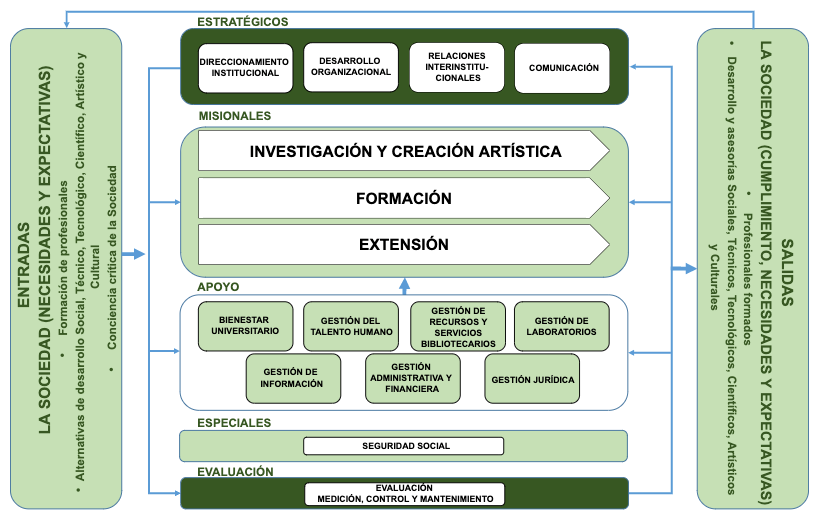
\includegraphics[width=1\linewidth]{Imagenes/figura_1} 

}

\caption{Mapa de procesos UNAL.}\label{fig:figura1}
\end{figure}

Fuente: \citet{Castro2021Jun}

\hypertarget{marco-conceptual}{%
\subsection{Marco conceptual}\label{marco-conceptual}}

\hypertarget{estaduxedsticas}{%
\subsubsection{Estadísticas}\label{estaduxedsticas}}

Las estadísticas son cifras de interés social e institucional las cuales se caracterizan, en el ámbito de lo público, principalmente por: ser construidas a partir de información poblacional disponible en registros administrativos y censos o inferida a través de estimaciones provenientes de muestras probabilísticas o no probabilísticas; permitir caracterizar/desagregar temporalmente, temáticamente y geográficamente rasgos de interés de los individuos que conforman las poblaciones o muestras de interés; hacer uso conceptos, estándares y nomenclaturas internacionales, nacionales e institucionales que favorezcan su interpretación y comparación; estar conformadas por cifras agregadas de naturaleza descriptiva derivadas de conteos o de mediciones; representar el presente y el pasado a través de la disposición de series de tiempo; ser susceptibles de ser representadas de manera tabular y gráfica (visualización); estar orientadas y delimitadas por normas; ser fácilmente interpretables y accesibles a través de múltiples mecanismos de disposición y divulgación; ser inclusivas; ser construidas a través de un proceso estadístico y finalmente, a partir de la comparación entre e intra poblaciones de las cifras agregadas, facilitar la creación de indicadores estadísticos.

\hypertarget{estaduxedsticas-oficiales}{%
\subsubsection{Estadísticas Oficiales}\label{estaduxedsticas-oficiales}}

Las estadísticas oficiales incluyen el subconjunto de estadísticas disponibles a nivel nacional y en cada una de las sedes de la Universidad asociadas a poblaciones de interés para la totalidad de procesos y acciones institucionales. Estas, más que emerger y pertenecer a un proceso particular, son útiles y requeridas por la totalidad de los procesos existentes a nivel institucional. Entre las principales categorías que agrupan las estadísticas oficiales de la Universidad tenemos: información de programas académicos, aspirantes y admitidos, matriculados, graduados, docentes, administrativos, investigación, extensión e innovación, capacidad financiera, etc. Las construcción, disposición y actualización de las estadísticas oficiales de la Universidad Nacional de Colombia, así como la disposición de los lineamientos conceptuales, metodológicos y técnicos requeridos para su gestión, se encuentra a cargo de las áreas de estadística adscritas a las direcciones de planeación y estadística en los niveles nacional y sede. La información estadística oficial de la Universidad, en su mayoría, se encuentra disponible o accesible a través del \href{http://estadisticas.unal.edu.co/home/}{sitio web institucional de estadísticas oficiales.}

\hypertarget{indicadores-estaduxedsticos}{%
\subsubsection{Indicadores Estadísticos}\label{indicadores-estaduxedsticos}}

Los indicadores estadísticos conservan, en términos generales, los mismos atributos que las estadísticas, pero a diferencia de estas, este tipo de mediciones requieren de un trabajo técnico de mayor complejidad que el exigido en las estadísticas. Este tipo de mediciones requieren de fórmulas o de procedimientos metodológicos para efectos del cálculo de la medida de interés y pueden ser de naturaleza simple como las tasas, las razones y las proporciones o complejos como los índices y las escalas.

\hypertarget{indicadores-de-gestiuxf3n}{%
\subsubsection{Indicadores de Gestión}\label{indicadores-de-gestiuxf3n}}

Los indicadores de gestión, a diferencia de las estadísticas y los indicadores estadísticos, se caracterizan porque miden el cumplimiento de una apuesta de futuro (meta) o el rango de desempeño asociado a una acción o conjunto de acciones pertenecientes a una política, proyecto o proceso institucional. Para su construcción y medición se requiere la disposición de líneas de base y, dependiendo del tipo de meta o rango de desempeño a ser monitoreado, pueden ser de diferentes tipos: flujo, acumulación, capacidad, reducción, reducción por periodo, stock. Los elementos conceptuales, metodológicos y técnicos que constituyen los indicadores de gestión o cumplimiento difieren de manera significativa respecto de los constitutivos de las estadísticas y los indicadores estadísticos.

\hypertarget{variable}{%
\subsubsection{Variable}\label{variable}}

Es una característica asociada a un ámbito de interés que puede variar y cuya variación adopta diversos posibles valores. Los valores asociados a una variable pueden medirse u observarse de manera directa -- variables observables - o indirecta -- variables no observables -.

\hypertarget{variables-observables}{%
\subsubsection{Variables observables}\label{variables-observables}}

Cualquier atributo o característica de fácil definición, medición y consenso dentro de un área, disciplina o teoría científica. Hacen referencia a algo que se sabe que existe y que se puede observar, manipular y medir de manera directa. La edad, el sexo o la profesión de una persona, son ejemplos de variables observables y de interés en el ámbito de la educación o las ciencias de la salud, por ejemplo.

\hypertarget{variables-no-observables}{%
\subsubsection{Variables no observables}\label{variables-no-observables}}

Cualquier entidad o categoría conceptual de difícil definición, medición y consenso dentro de un área, disciplina o teoría científica. También conocidas como variables latentes o constructos, hacen referencia a algo que se sabe que existe pero que no se puede observar, manipular y medir de manera directa --no observables-. La inteligencia, la personalidad, la creatividad, el bienestar individual o social, son algunos ejemplos de constructos de interés académico para disciplinas como la psicología, la economía o la sociología; en contraste, por ejemplo, la satisfacción del usuario, lo es para el ámbito de la gestión administrativa.

\hypertarget{documentos-de-referencia}{%
\subsection{Documentos de referencia}\label{documentos-de-referencia}}

\begin{itemize}
\tightlist
\item
  \citet{bonnefoy2005indicadores}
\item
  \citet{coneval2013manual}
\item
  \citet{sanchez2018guia}
\item
  \citet{dane2014guia}
\item
  \citet{publica2015guia}
\end{itemize}

\hypertarget{condiciones-generales}{%
\subsection{Condiciones generales}\label{condiciones-generales}}

\hypertarget{objetivos-de-la-cuantificaciuxf3n-mediciuxf3n-y-seguimiento-a-la-gestiuxf3n-de-los-procesos}{%
\subsubsection{Objetivos de la cuantificación, medición y seguimiento a la gestión de los procesos}\label{objetivos-de-la-cuantificaciuxf3n-mediciuxf3n-y-seguimiento-a-la-gestiuxf3n-de-los-procesos}}

\begin{itemize}
\item
  Determinar el nivel de desempeño de los procesos de la UNAL respecto a los objetivos y las metas fijadas, para establecer que tan cerca o lejos se encuentra de su cumplimiento.
\item
  Tomar decisiones a partir del análisis de los resultados obtenidos bien sea para mantener, prevenir o mejorar el estado actual de los procesos con respecto a sus objetivos y metas.
\item
  Presentar información que agregue valor a la gestión y que permita la rendición de cuentas a las partes interesadas (usuarios, directivos, entes de control internos y externos) frente a la aplicación de los recursos en la ejecución de los procesos, como muestra de transparencia en el ejercicio de la función pública.
\end{itemize}

\hypertarget{normativa-aplicable}{%
\subsubsection{Normativa aplicable}\label{normativa-aplicable}}

\begin{table}

\caption{\label{tab:unnamed-chunk-3}*Marco normativo aplicable a la cuantificación, medición y seguimiento a la gestión de los procesos UNAL*}
\centering
\begin{tabular}[t]{l|l|l|l}
\hline
Tipo de documento & Titulo de documento & Interna & Externa\\
\hline
Constitución Política de Colombia & TÍTULO XII. DEL RÉGIMEN ECONÓMICO Y DE LA HACIENDA PÚBLICA. Capítulo 2. De los planes de desarrollo. Art 343. La entidad nacional de planeación que señale la ley, tendrá a su cargo el diseño y la organización de los sistemas de evaluación de gestión y resultados de la administración pública, tanto en lo relacionado con políticas como con proyectos de inversión, en las condiciones que ella determine. &  & X\\
\hline
Ley 87 de 1993 & *“Por la cual se establecen normas para el ejercicio del control interno en las entidades y organismos del Estado y se dictan otras disposiciones”*. Art 2. Objetivos del Sistema de Control Interno. Literal d) Garantizar la correcta evaluación y seguimiento de la gestión organizacional. Art 4. Elementos para el Sistema de Control Interno. Literal j) Organización de métodos confiables para la evaluación de la gestión. &  & X\\
\hline
Ley 872 de 2003 & Por la cual se crea el sistema de gestión de la calidad en la Rama Ejecutiva del Poder Público y en otras entidades prestadoras de servicios. Art 4. Requisitos para su implementación. Literal h) Realizar el seguimiento, el análisis y la medición de estos procesos. PARÁGRAFO 1º. Este sistema tendrá como base fundamental el diseño de indicadores que permitan, como mínimo, medir variables de eficiencia, de resultado y de impacto que faciliten el seguimiento por parte de los ciudadanos y de los organismos de control, los cuales estarán a disposición de los usuarios o destinatarios y serán publicados de manera permanente en las páginas electrónicas de cada una de las entidades cuando cuenten con ellas. &  & X\\
\hline
Decreto 1083 de 2015 & *“Por medio del cual se expide el Decreto Único Reglamentario del Sector de Función Pública”*. Título 21. Sistema de Control Interno. Capítulo 3. Sistema Institucional y Nacional de Control Interno.ARTÍCULO 2.2.21.3.4 Planeación. Parágrafo. Literal d) La Oficina de Control Interno o quien haga sus veces: Evalúa el proceso de planeación, en toda su extensión; implica, entre otras cosas y con base en los resultados obtenidos en la aplicación de los indicadores definidos, un análisis objetivo de aquellas variables y/o factores que se consideren influyentes en los resultados logrados o en el desvío de los avances. La identificación de estas variables, su comportamiento y su respectivo análisis permite que la formulación de las recomendaciones de ajuste o mejoramiento al proceso, se realice sobre soportes y criterios válidos y visibles fortaleciendo así la función asesora de estas oficinas. &  & X\\
\hline
Decreto 1499 de 2017 & *“Por medio del cual se modifica el Decreto 1083 de 2015, Decreto Único Reglamentario del Sector Función Pública, en lo relacionado con el Sistema de Gestión establecido en el artículo 133 de la Ley 1753 de 2015”* Capítulo 2. Politicas de Gestión y Desempeño Institucional. ARTÍCULO  2.2.22.2.1. Políticas de Gestión y Desempeño Institucional. Numeral 16. Seguimiento y evaluación del desempeño institucional. &  & X\\
\hline
Resolución 316 de 2018 & *“Por la cual se actualiza el Sistema de Control Interno de la Universidad Nacional de Colombia, y se derogan las Resoluciones de Rectoría 1428 de 2006 y 139 de 2018”*. Art. 5. Objetivos específicos del Sistema de Control Interno. Numeral 5.3 Objetivos de control de evaluación y seguimiento. Literal  a) Garantizar que el Sistema de Control Interno disponga de sus propios mecanismos de verificación y evaluación, que faciliten en tiempo real, realizar seguimiento a la gestión de la Universidad por parte de los diferentes niveles de autoridad, permitiendo acciones oportunas de prevención, corrección y de mejoramiento… e) Garantizar razonablemente la correcta evaluación y seguimiento de la gestión académico administrativa… Art 11. Responsabilidad del Sistema de Gestión. Literal a) Apoyar el proceso de implementación y fortalecimiento continuo del Modelo Estándar de Control Interno bajo las orientaciones del representante de la dirección… d) Trabajar en coordinación con los servidores designados por las otras áreas en aquellas actividades requeridas para la implementación y fortalecimiento continuo del Modelo Estándar de Control Interno. & X & \\
\hline
Resolución 1528 de 2018 & *“Por la cual se define, se estructura y se establecen roles y responsabilidades del Sistema Integrado de Gestión Académico, Administrativo y Ambiental en la Universidad Nacional de Colombia y se derogan las Resoluciones que le sean contrarias”* & X & \\
\hline
\end{tabular}
\end{table}

\hypertarget{roles-y-responsabilidades-en-la-cuantificaciuxf3n-mediciuxf3n-y-seguimiento-a-la-gestiuxf3n-de-los-procesos}{%
\subsubsection{Roles y responsabilidades en la cuantificación, medición y seguimiento a la gestión de los procesos}\label{roles-y-responsabilidades-en-la-cuantificaciuxf3n-mediciuxf3n-y-seguimiento-a-la-gestiuxf3n-de-los-procesos}}

\begin{table}

\caption{\label{tab:tabla2}*Roles en la cuantificación, medición y seguimiento a la gestión de los procesos en la UNAL*}
\centering
\begin{tabular}[t]{l|l|l|l}
\hline
Sigla & Rol & Descripción & Referencia\\
\hline
CGR & Contraloría General de la República & Ejercer control fiscal de la institución incluyendo el control financiero, de gestión y de resultados, fundado en la eficacia, la economía, la equidad y la valoración de los costos ambientales. & Constitución Política de 1991 Art 267 inciso 3\\
\hline
CNCSCI & Comite´ Nacional de Coordinación del Sistema de Control Interno & Evaluar el estado del Sistema de Control Interno de acuerdo con las características propias de la Universidad Nacional de Colombia y aprobar las modificaciones, actualizaciones y acciones de fortalecimiento del sistema a partir de la normatividad vigente, los informes presentados por el jefe de control interno o quien haga sus veces, organismos de control y las recomendaciones del Sistema Integrado de Gestión Académico Administrativo y Ambiental, o quien haga sus veces. & Resolución 316 de 2018 Art 8. Numeral 8.1. Literal a).\\
\hline
CSIGA & Comité Directivo SIGA & Definir lineamientos y directrices que incorporen de manera estratégica y unificada en todas las Sedes de la Universidad Nacional de Colombia, la apropiación, implementación, evaluación, seguimiento y mejora del  componente cuantificación, medición y seguimiento  a la gestión de los procesos, que hace parte del SIGA. & Resolución 1528 de 2018. Capítulo I. Del nivel nacional. Art 9. Literal b.\\
\hline
ONCI & Oficina Nacional de Control Interno & Evaluar la planeación, ejecución y control en la gestión de los procesos, programas, planes y proyectos de la Universidad, desde el rol del evaluador independiente. Su finalidad es generar información, recomendaciones, alertas y aprendizajes que contribuyan al mejoramiento de la gestión. & Resolución 316 de 2018\\
\hline
DNPE & Dirección Nacional de Planeación y Estadística & • Brindar apoyo y acompañamiento metodológico a la VRG en la adecuación del modelo de medición, cuantificación y seguimiento a la gestión de los procesos de acuerdo a las necesidades de la UNAL. <br> •   Suministrar las cifras oficiales de la UNAL requeridas en el proceso de construcción de los indicadores de gestión de los procesos. & Acuerdo 238 de 2017 Resolución 383 de 2014 de Rectoría\\
\hline
VRS/DS & Vicerrectori´a de Sede / Direccio´n de Sede & Mantenerse informado de los lineamientos para la cuantificación, medición y seguimiento a la gestión de los procesos y su ejecucio´n al interior de la Sede. & Resolución 1528 de 2018\\
\hline
LSNN & Líder SIGA NN & • Formular una metodología e instrumentos para la cuantificación, medición y seguimiento a la gestión de los procesos en la UNAL. <br> • Proporcionar entrenamiento a los Li´deres del NN y Sedes en la metodologi´a para la cuantificación, medición y seguimiento a la gestión de los procesos de la UNAL. <br> • Coordinar la ejecución de los lineamientos para la cuantificación, medición y seguimiento a la gestión de los procesos con los Li´deres del NN. <br >*   Asistir a los Li´deres del NN para la aplicación de la metodología para la cuantificación, medición y seguimiento a la gestión de los procesos.  <br> • Consolidar y presentar los resultados de la medición de la gestión de los procesos a las partes interesadas, a partir de la informacio´n proporcionada por los Li´deres de los mismos en el NN.   <br>• Desarrollar las actividades que le corresponden al Li´der del Nivel Nacional para los procesos que no cuentan con esta figura en las Sedes. <br> • Responder a los requerimientos de entes de control tanto internos como externos para demostrar la conformidad de la cuantificación, medición y seguimiento a la gestión de los procesos de la UNAL con los compromisos tanto normativos como institucionales. & Resolución 1528 de 2018\\
\hline
CSS & Coordinador SGC Sede & • Replicar la metodología para la cuantificación, medición y seguimiento a la gestión de los procesos UNAL a los líderes de los mismo en el nivel de Sede. <br> • Coordinar la ejecución de los lineamientos para la cuantificación, medición y seguimiento a la gestión de los procesos en la UNAL, con los Líderes de los mismos en la Sede, Facultad, Centro, Instituto o Laboratorio, según el caso. <br> • Asistir a los Líderes de los procesos de la Sede para el desarrollo de las diferentes etapas de la cuantificación, medición y seguimiento a su gestión. <br> • Velar por que los Li´deres de los procesos de la Sede entreguen la informacio´n producto del desarrollo de las etapas de la gestio´n de los riesgos oportunamente a sus pares en el NN. <br> • Revisar la calidad de la información de la cuantificación, medición y seguimiento a la gestión de los procesos, reportada por los líderes en la sede, para verificar que guarde coherencia con la metodología definida por la UNAL <br> • Consolidar la información de cuantificiación, medición y seguimiento a la gestión de los procesos generada en la sede. <br> • Generar los reportes e informes de gestión relacionados con la medición de indicadores de procesos correspondiente a la sede. <br> • Responder a los requerimientos de entes de control tanto internos como externos para demostrar la conformidad de la cuantificación, medición y seguimiento a la gestión de los procesos de la UNAL con los compromisos tanto normativos como institucionales. <br> & Resolución 1528 de 2018\\
\hline
LPNN & Líder de proceso nivel nacional & • Desarrollar las diferentes etapas para la cuantificación, medición y seguimiento a la gestión del proceso de manera participativa con sus pares de acuerdo a su nivel de aplicación (Sede, Facultad, Centro, Instituto o Laboratorio). <br> • Consolidar y presentar los resultados del desarrollo de las diferentes etapas para la cuantificación, medición y seguimiento a la gestión del proceso a las partes interesadas (Líder SIGA NN, Líder proceso Sede y auditores internos o externos). <br> • Responder a los requerimientos de entes de control tanto internos como externos para demostrar la conformidad de la cuantificación, medición y seguimiento a la gestión de los procesos de la UNAL con los compromisos tanto normativos como institucionales. & Resolución 1528 de 2018\\
\hline
LPS & Líder de proceso sede & • Desarrollar las diferentes etapas para la cuantificación, medición y seguimiento a la gestión del proceso de manera participativa con sus pares de acuerdo a su nivel de aplicación (Nivel Nacional, Facultad, Centro, Instituto o Laboratorio). <br> • Consolidar y presentar los resultados del desarrollo de las diferentes etapas para la cuantificación, medición y seguimiento a la gestión del proceso a las partes interesadas (Líder proceso en el nivel nacional, Líder de proceso en Facultad, Centro, Instituto o Laboratorio y auditores internos o externos). <br> • Responder a los requerimientos de entes de control tanto internos como externos para demostrar la conformidad de la cuantificación, medición y seguimiento a la gestión de los procesos de la UNAL con los compromisos tanto normativos como institucionales. & Resolución 1528 de 2018\\
\hline
LPF/C/I/L & Líder de proceso Facultad, Centro, Instituto o Laboratorio & • Desarrollar las diferentes etapas para la cuantificación, medición y seguimiento a la gestión del proceso de manera participativa con sus pares de acuerdo a su nivel de aplicación (Nivel Nacional, Sede). <br> • Consolidar y presentar los resultados del desarrollo de las diferentes etapas para la cuantificación, medición y seguimiento a la gestión del proceso a las partes interesadas (Líder de proceso en el nivel nacional, Líder de proceso en Sede y auditores internos o externos). <br> • Responder a los requerimientos de entes de control tanto internos como externos para demostrar la conformidad de la cuantificación, medición y seguimiento a la gestión de los procesos de la UNAL con los compromisos tanto normativos como institucionales. & Resolución 1528 de 2018\\
\hline
AE/AI & Auditor externo o interno & Evaluar los resultados de la cuantificación, medición y seguimiento de la gestión de los procesos de la UNAL de acuerdo con las evidencias recopiladas en contraste con los criterios de auditoria establecidos. & NTC ISO 9001: 2015 NTC ISO 19011: 2018\\
\hline
\end{tabular}
\end{table}

\hypertarget{modelo-de-gestiuxf3n-de-la-informaciuxf3n-en-la-universidad-nacional-de-colombia}{%
\chapter{Modelo de gestión de la información en la Universidad Nacional de Colombia}\label{modelo-de-gestiuxf3n-de-la-informaciuxf3n-en-la-universidad-nacional-de-colombia}}

La gestión de la información disponible al interior de las organizaciones en general y de las universidades en particular es uno de los grandes retos que estas enfrentan en la actualidad. ¿Cómo entender la categoría información a nivel institucional?, ¿de qué tipo de datos estamos hablando a la hora de gestionar la información?, ¿qué datos poseemos, quién los administra y qué calidad presentan?, ¿quién es el dueño de los datos y bajo qué parámetros o reglas estos pueden ser gestionados?, ¿los diferentes tipos de datos existentes en las organizaciones implican formas diferentes para su gestión?, ¿qué productos o servicios se pueden derivar a partir de una correcta gestión de la información disponible?, ¿qué papel desempeñan las estadísticas y los indicadores de gestión, por ejemplo, en el ámbito de la información institucional?, etc. son algunas de las preguntas que enfrentan en la actualidad aquellas organizaciones que consideran sus datos como un activo institucional y su correcta gestión como uno de las acciones a desarrollar.

En este contexto, la Universidad Nacional de Colombia, durante los últimos años \footnote{Ejemplos de esta importancia, en años anteriores, por ejemplo, se ven reflejados en la gestión de la información estadística la cual, además de venirse desarrollando de manera permanente en la Universidad desde aproximadamente el año 1965, se formalizó durante los últimos años con la creación de la Oficina Nacional de estadística adscrita a la Dirección Nacional de Planeación y Estadística. No menos importante, ha resultado la importancia que se le ha dado a la medición a nivel institucional y en términos de gestión desde que esta incursionó en la implementación de su Sistema de Calidad (antes llamado SIMEGE y hoy denominado SIGA).} y, en especial, a partir del actual Plan Global de Desarrollo 2019-2021 \emph{``Proyecto Cultural y Colectivo de Nación''}, de la reciente creación de la Dirección Nacional de Estrategia Digital DNED y dentro de esta, con la creación de la Oficina de Gestión de la Información, no sólo ha considerado sus datos como un activo institucional, sino que ha venido generando las condiciones para una correcta gestión de los mismos. En este contexto, en la actualidad la institución se encuentra en el proceso de construcción y disposición de un modelo que oriente la gestión de la información disponible a nivel institucional en donde, los indicadores de gestión, que conforman el objeto de esta guía, tienen un espacio definido.

La Figura \ref{fig:figura2}, presenta una primera aproximación a los componentes, los instrumentos y las herramientas que hacen parte de una primera propuesta de modelo para la gestión de la información a nivel institucional. Este modelo, como se observa en la Figura, inicia con la importancia de entender los datos como un bien/activo institucional que presenta, desde una perspectiva económica, una característica de no rivalidad \footnote{Un bien no rival es aquel cuyo uso para un propósito no impide que los mismos sean utilizados para otros propósitos. Desde luego, los datos, al poderse emplear en múltiples propósitos, los hace bienes o activos de tipo no rival.}. En segundo lugar, los datos en la actualidad pueden ser clasificados en: estructurados, semiestructurados y no estructurados.

Las diferentes tipologías de los datos se materializan a nivel de la Universidad en necesidades o demandas de información las cuales pueden ser de tipo externo, internos e incluso algunas para las cuales aún no existen datos disponibles. Para dar respuesta a las necesidades actualmente existentes a nivel institucional en materia de información, en principio y como se observa en la parte derecha de la Figura \ref{fig:figura2}, se propone que el modelo de gestión de la información institucional esté conformado por 4 servicios de información: estadísticas e indicadores, datos abiertos, intercambio de datos y el servicio de analítica e inteligencia institucional.

El modelo propuesto a su vez está atravesado por 4 componentes transversales que impactan la gestión de la información en la Universidad. La calidad de los datos disponibles y su aseguramiento en el futuro, la seguridad de los datos y de la información institucional, la gobernabilidad de los datos disponibles, así como el reconocimiento de los aspectos legales involucrados a la hora de gestionar datos, se convierten en 4 elementos que atraviesan la gestión de la información institucional.

\begin{figure}

{\centering 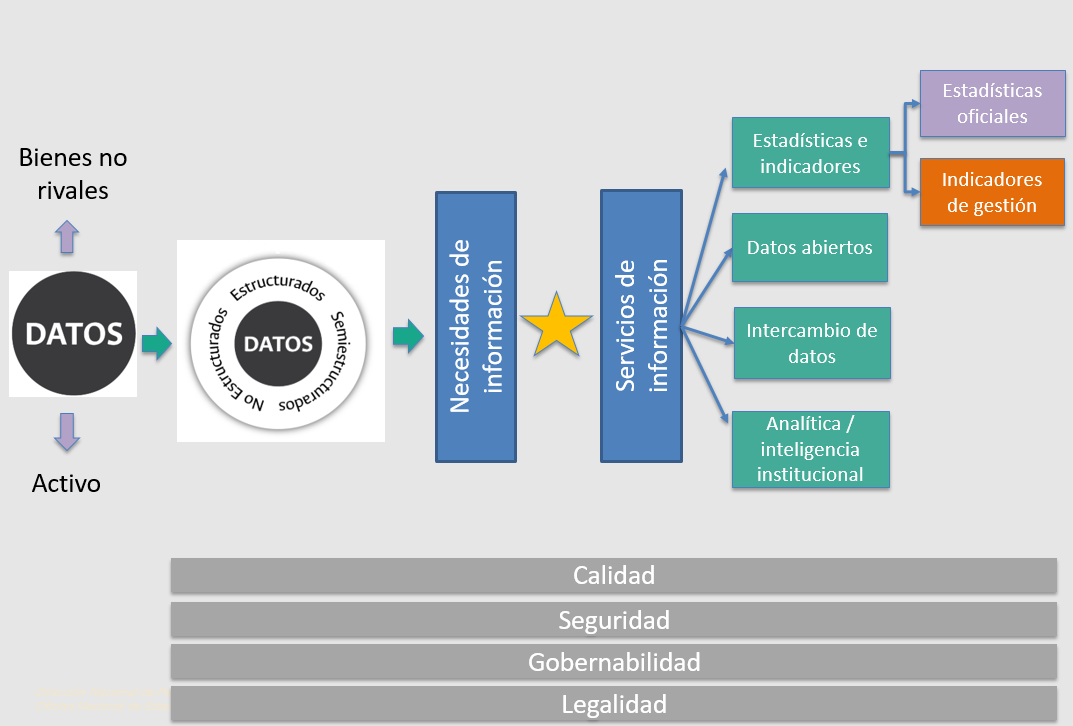
\includegraphics[width=1\linewidth]{Imagenes/figura_2} 

}

\caption{Modelo de Gestión de la Información en la UNAL}\label{fig:figura2}
\end{figure}

Los indicadores de gestión, que hacen parte del objeto de esta guía, en el marco de la gestión de la información institucional (\emph{Ver Figura \ref{fig:figura2}: Modelo de Gestión de la Información en la UNAL}) se ubican en el contexto de los servicios de información institucional propuestos y, en específico, dentro del componente de estadísticas e indicadores institucionales.

\hypertarget{metodologuxeda-para-la-definiciuxf3n-de-indicadores-de-gestiuxf3n-en-los-procesos-de-la-unal}{%
\chapter{Metodología para la definición de indicadores de gestión en los procesos de la UNAL}\label{metodologuxeda-para-la-definiciuxf3n-de-indicadores-de-gestiuxf3n-en-los-procesos-de-la-unal}}

En múltiples escenarios se ha reconocido el uso de los indicadores de gestión como una de las formas más simples en las que cualquier entidad puede transformar sus datos en información útil para la toma de decisiones, debido principalmente a su enorme capacidad para comunicar el grado de cumplimiento de metas y objetivos institucionales. De ahí parte la necesidad de establecer a nivel institucional un método claro y estructurado que permita la cuantificación, medición y seguimiento al desempeño de los procesos, a través de instrumentos objetivos, sin perder de vista el enorme desafío que representa el separar los datos útiles de los irrelevantes, debido a los altos volúmenes de información que se generan constantemente en la operación cotidiana de la Universidad.

Es por esto que a través de una revisión sistemática de referentes como el Departamento Administrativo de la Función Pública DAFP, el Departamento Administrativo Nacional de Estadística DANE, el Departamento Nacional de Planeación DNP, la Comisión Económica para América Latina y el Caribe CEPAL y el Consejo Nacional de Evaluación de la Política de Desarrollo Social CONEVAL de México, se presenta el método para la formulación y aplicación de los indicadores de gestión en los procesos adoptado por la UNAL, compuesto por 6 fases secuenciales (\emph{Ver Figura \ref{fig:figura3}: Diagrama de flujo para la cuantificación, medición y seguimiento a la gestión de los procesos UNAL}) que se detallan en los siguientes apartados de la presente guía:

\begin{figure}

{\centering 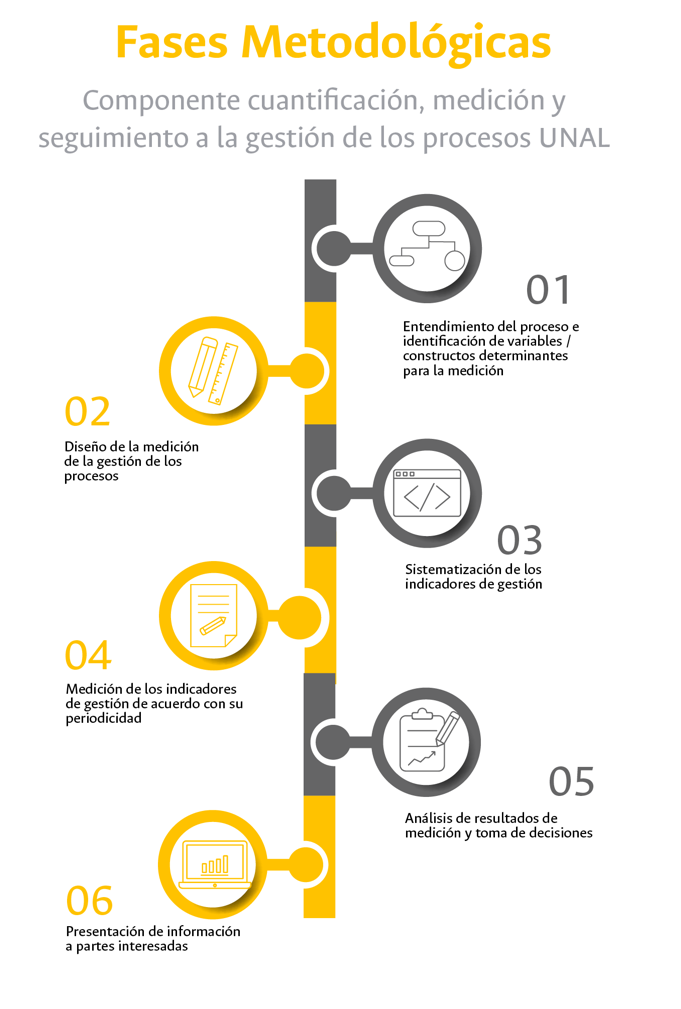
\includegraphics[width=0.7\linewidth]{Imagenes/figura_3} 

}

\caption{Diagrama de flujo para la cuantificación, medición y seguimiento a la gestión de los procesos UNAL}\label{fig:figura3}
\end{figure}

\hypertarget{entendimiento-del-proceso-e-identificaciuxf3n-de-variables-observables-y-no-observables-determinantes-para-la-mediciuxf3n}{%
\section{Entendimiento del proceso e identificación de variables observables y no observables determinantes para la medición}\label{entendimiento-del-proceso-e-identificaciuxf3n-de-variables-observables-y-no-observables-determinantes-para-la-mediciuxf3n}}

Antes de iniciar con la definición de los indicadores de gestión asociados a un proceso en particular, es necesario hacer un análisis exhaustivo de aquello que se pretende medir. Por lo que se requiere un entendimiento de dicho proceso desagregándolo en sus diferentes componentes, los cuales se encuentren definidos en las siguientes fuentes de información:

\begin{itemize}
\item
  Caracterización de proceso: En este documento se presenta el objetivo con el cual se establece la intensión y finalidad hacia la que se dirigen los recursos y esfuerzos involucrados en su operación de manera descriptiva y concreta, al tiempo que se describen sus entradas o insumos requeridos, los productos o servicios que se espera obtener, las diferentes fases del ciclo PHVA y los responsables de su ejecución.
\item
  Las metas y resultados que se propone alcanzar los cuales se encuentran inmersos tanto en los procedimientos como en planes y proyectos.
\item
  Las herramientas tanto informáticas como documentales (formatos) en las que se registran los datos que dan cuenta de la ejecución del proceso para establecer posibles fuentes de información.
\item
  La caracterización de usuarios y partes interesadas en la que se establecen cuales son sus grupos de interés con sus necesidades y expectativas, así como los productos y servicios esperados.
\item
  La matriz DOFA con el análisis de contexto en el que se enuncian sus debilidades, oportunidades, fortalezas y amenazas. En la esfera externa del proceso se pueden identificar las habilidades que se requieren para se exitoso, mientras que a nivel interno se pueden identificar las situaciones que pueden influir en su éxito o fracaso.
\item
  El normograma con la normativa aplicable en la que se establecen aquellos aspectos que el proceso debe cumplir en términos legales.
\end{itemize}

Una vez se tiene claridad de las características del proceso en particular, se requiere establecer cuales variables observables y no observables son determinantes para su medición, es decir, cuales son los atributos, aspectos o condiciones tanto internas como externas que se pueden influenciar a través de decisiones al tiempo que afectan significativamente el cumplimiento de su objetivo. En otras palabras, se podría decir que si los objetivos son los fines hacia los cuales se dirigen los esfuerzos y recursos institucionales, las variables observables y no observables determinantes para su medición son los medios a través de los cuales dichos fines se logran.

A partir de este análisis es posible obtener un listado de aspectos más o menos numeroso, el cual debe ser priorizado y calificado en relación con la relevancia que tiene para el proceso con el fin de decantar la información inicial y enfocarse en aquellos que tiene mayor incidencia en su desempeño global. Para lograrlo se debe evitar que las variables resultantes contengan elementos redundantes y procurar porque sean coherentes entre si para lograr un balance entre la cantidad y la calidad de la información.

En la práctica, para el desarrollo de esta fase se requerirán sesiones de trabajo con funcionarios involucrados en el proceso, quienes de acuerdo con su nivel de experiencia y conocimiento podrán aportar a la construcción del listado de variables observables y no observables y su posterior depuración, las cuales serán usadas como punto de partida para la definición de los indicadores de gestión.

Si bien las variables observables y no observables determinantes de medición son específicas para cada objetivo de proceso y cada tipo de entidad a continuación, se enuncian posibles categorías en las que estas se pueden clasificar acompañadas de ejemplos relacionados con el contexto de la Universidad:

\begin{itemize}
\item
  \emph{Tiempo:} Oportunidad en la prestación del servicio.
\item
  \emph{Cobertura:} Incremento en el número de estudiantes matriculados, número de beneficiarios de programas de bienestar, número de usuarios de un servicio específico.
\item
  \emph{Financiero:} Costos de operación.
\item
  \emph{Cumplimiento:} Avance en las acciones o actividades programadas, ejecuciones de actividades específicas.
\item
  \emph{Calidad:} Número de devoluciones, reprocesos, acreditación de programas curriculares, incumplimiento de estándares o especificaciones.
\item
  \emph{Cantidad:} Productos de investigación, publicaciones, patentes.
\item
  \emph{Constructos o conceptos:} Competencia del talento humano, comunicación organizacional, desarrollo y desempeño docente.
\item
  \emph{Otras:} Deserción estudiantil, repetición de materias, alianzas interinstitucionales y empresariales, intercambio estudiantil o docente.
\end{itemize}

Así mismo en la Figura \ref{fig:figura4} se proponen 4 perspectivas o dimensiones en las que se podría enmarcar el desempeño de un proceso en la UNAL (véase \citet{bolborici2012aplicacion}) , de tal manera que se pueda hacer un análisis desde múltiples puntos de vista para traducir sus objetivos en acciones concretas y medibles orientadas a la creación de valor, facilitando la identificación de las variables determinantes de medición:

\begin{figure}

{\centering 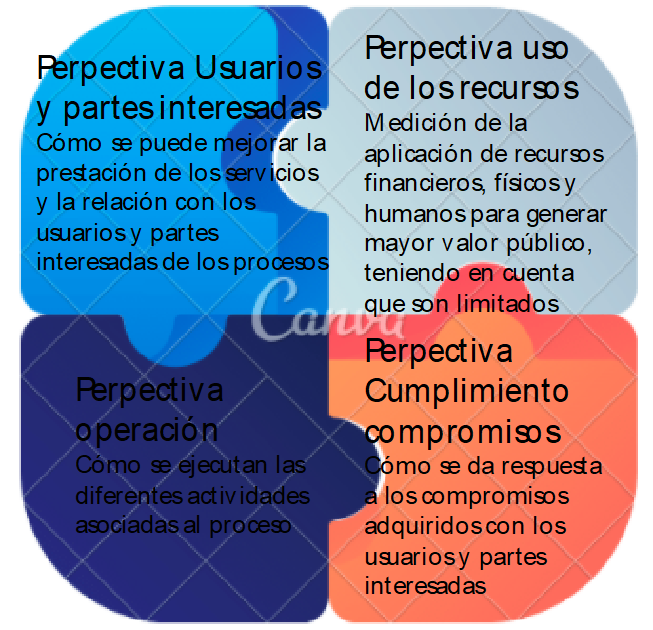
\includegraphics[width=0.6\linewidth]{Imagenes/figura_4} 

}

\caption{Perspectivas para la ubicación de las variables determinantes de medición }\label{fig:figura4}
\end{figure}

En el \protect\hyperlink{anexos}{anexo 1} de esta guía se propone un método de evaluación de la criticidad de las variables determinantes de medición para su priorización de acuerdo con tres criterios como son el impacto que la variable tiene sobre el objetivo del proceso, la confiabilidad de los datos para su medición y el último es la capacidad de gestión sobre la variable. Este método podrá utilizarse para facilitar la selección de variables asociadas a un proceso en caso de tener un listado numeroso.

Por otra parte conviene mencionar en este apartado que en los diferentes modelos estudiados para la construcción de esta guía se presentan diversas estructuras para la clasificación de los indicadores de gestión, como el caso de la Función \citet{publica2015guia}, que muestra un enfoque desde la visión de la cadena de valor, donde se ubican las tipologías de indicadores de acuerdo a su relación con cada eslabón de dicha cadena (\emph{Ver figura \ref{fig:figura5}: Categoría de indicadores de acuerdo a su ubicación en la cadena de valor público propuesta por el DAFP}). En esta jerarquía se proponen indicadores desde el punto de vista del desempeño (economía, eficiencia, eficacia, efectividad y calidad), y desde el punto de vista de resultados (insumo, proceso, producto, resultados finales e impacto) asociados a un flujo de información que se dirige en el sentido de la operación de los procesos (de izquierda a derecha).

\begin{figure}

{\centering 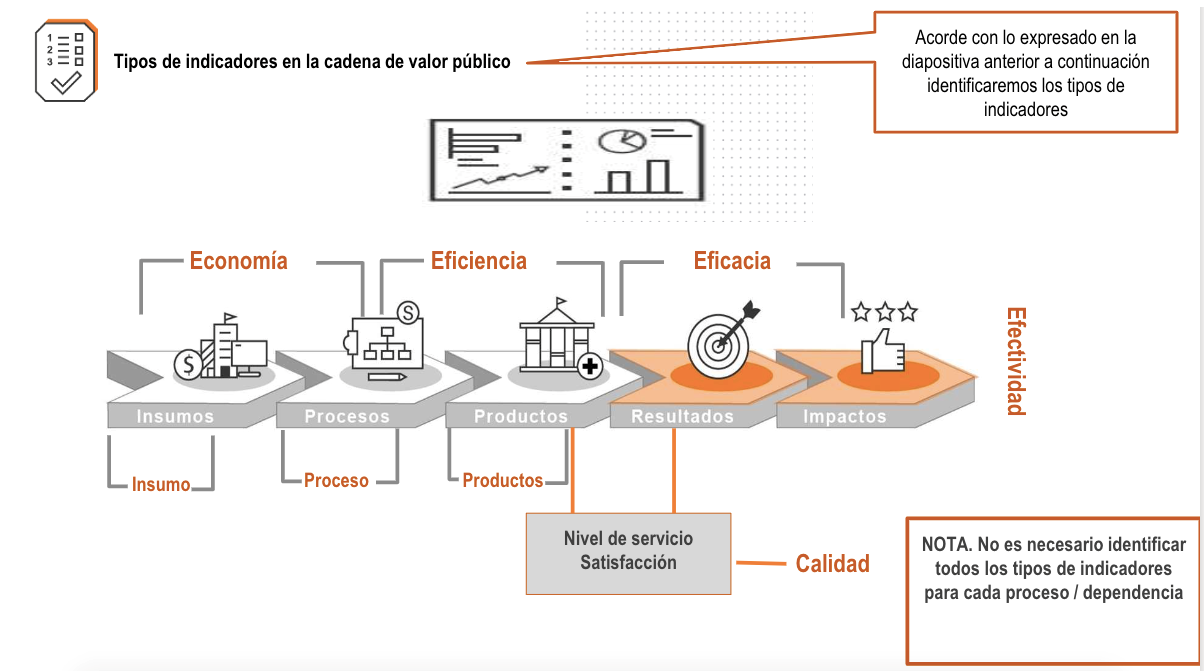
\includegraphics[width=0.85\linewidth]{Imagenes/figura_5} 

}

\caption{Categoría de indicadores de acuerdo a su ubicación en la cadena de valor público propuesta por el DAFP}\label{fig:figura5}
\end{figure}

Tomado de \citet{publica2015guia}.

De modo similar la guía del Departamento Nacional de Planeación (\citet{sanchez2018guia}) propone una clasificación de los indicadores asociada a la cadena de generación de valor público (\emph{Ver figura \ref{fig:figura6}: Categorías de indicadores con base en la cadena de valor de acuerdo al DNP}), donde se relacionan los insumos (factores de producción) con actividades a través de las cuales sufren un proceso de transformación para la generación de bienes o la prestación de servicios (productos) que finalmente conllevan al bienestar de los usuarios finales (resultados). La estructura de esta categorización de indicadores es tipo embudo en la que se inicia de arriba hacia abajo con tipologías que van de mayor a menor complejidad en su estructura.

\begin{figure}

{\centering 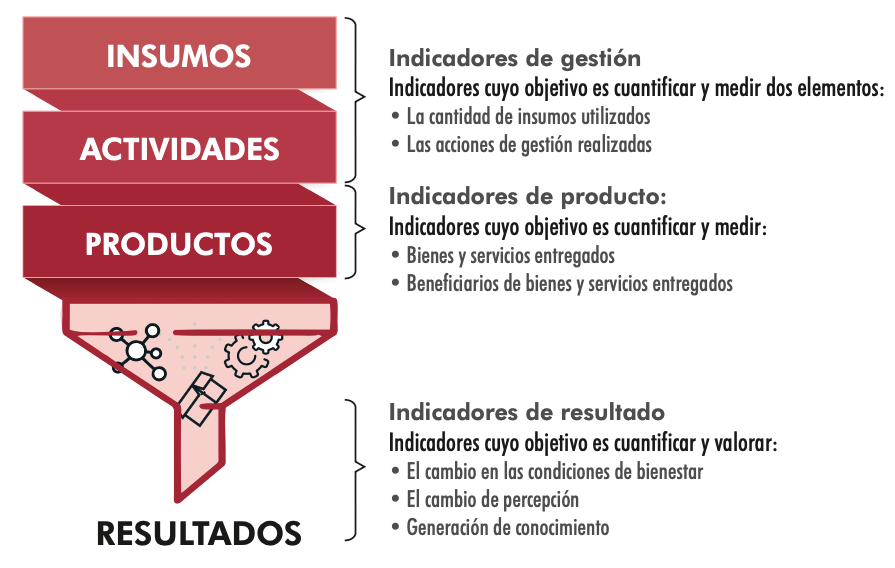
\includegraphics[width=0.7\linewidth]{Imagenes/figura_6} 

}

\caption{Categorías de indicadores con base en la cadena de valor de acuerdo con el DNP}\label{fig:figura6}
\end{figure}

Tomado de \citet{sanchez2018guia}.

Por su parte, la guía para la construcción de indicadores del DANE, según \citet{dane2014guia} establece que existen cuatro tipos de clasificaciones comunes: según medición, nivel de intervención, jerarquía y calidad (\emph{Ver figura \ref{fig:figura7}: Interrelación entre indicadores, según nivel de resultados y jerarquía}), haciendo la salvedad que no son excluyentes entre si y que se pueden usar de acuerdo con las necesidades de los procesos estadísticos de las entidades. Los indicadores según su medición se categorizan en cuantitativos y cualitativos, en cuanto al nivel de intervención se dispone de las tipologías impacto, resultado, producto, proceso e insumo, según la jerarquía se tienen indicadores de gestión y estratégicos y finalmente se tienen las categorías de indicadores según la calidad como son eficacia, eficiencia y efectividad. En este caso la estructura es piramidal de abajo hacia arriba del menos al más estratégico de acuerdo con su relación con la jerarquía de los objetivos de la entidad.

\begin{figure}

{\centering 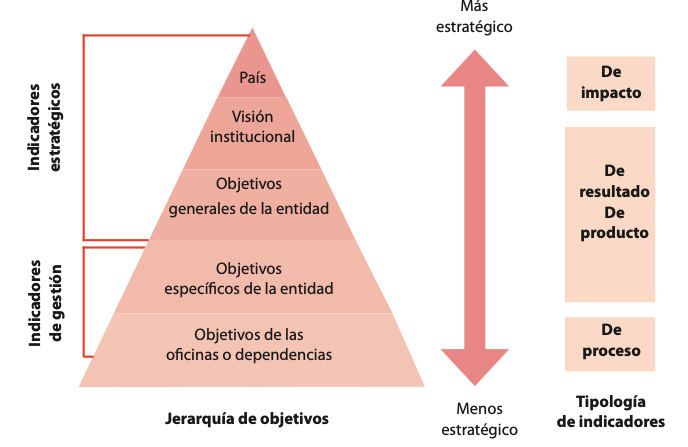
\includegraphics[width=0.7\linewidth]{Imagenes/figura_7} 

}

\caption{: Interrelación entre indicadores, según nivel de resultados y jerarquía}\label{fig:figura7}
\end{figure}

Tomado de \citet{dane2014guia}.

Como otro referente se tiene la taxonomía propuesta por la CEPAL en su manual de indicadores para el sector público que incluye dos formas de clasificación diferentes (véase \citet{bonnefoy2005indicadores}), la primera a indicadores desde el punto de vista de la actuación pública en la generación de productos como son insumo, procesos o actividades, productos y resultados finales y la segunda los cataloga de acuerdo con el desempeño es estas actuaciones en las dimensiones de eficiencia, eficacia, calidad y economía. Gráficamente esta distribución se presenta como una red de interrelaciones entre ambas categorías de indicadores desde la perspectiva del proceso productivo integrado a los niveles de servicio, al uso de recursos y la satisfacción de los usuarios (\emph{Ver figura \ref{fig:figura8}: Taxonomía de indicadores desde la perspectiva del proceso productivo según CEPAL}).

\begin{figure}

{\centering 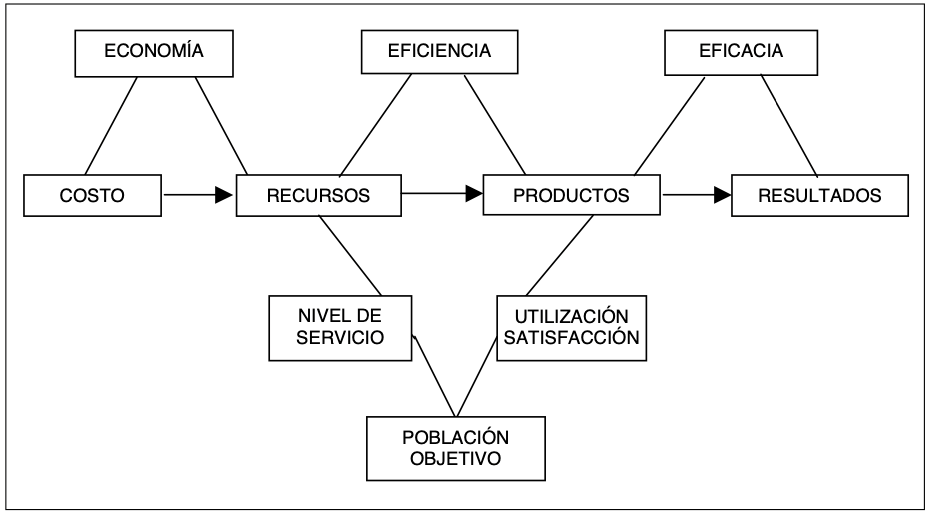
\includegraphics[width=0.7\linewidth]{Imagenes/figura_8} 

}

\caption{: Taxonomía de indicadores desde la perspectiva del proceso productivo según CEPAL}\label{fig:figura8}
\end{figure}

Tomado de \citet{bonnefoy2005indicadores}.

Finalmente, según \citet{coneval2013manual} considera cuatro dimensiones de desempeño: eficacia, eficiencia, calidad y economía que permiten medir el cumplimiento de un objetivo en relación con el nivel de logro que se espera alcanzar, de tal manera que el análisis desde diversos ángulos muestre una valoración integral del mismo (\emph{Ver figura \ref{fig:figura9}: Dimensiones sugeridas de los indicadores CONEVAL}). Este enfoque relaciona los momentos en los que se realiza la medición (cuándo) con aquello que se está midiendo (qué) para establecer que tipo de indicador es recomendable.

\begin{figure}

{\centering 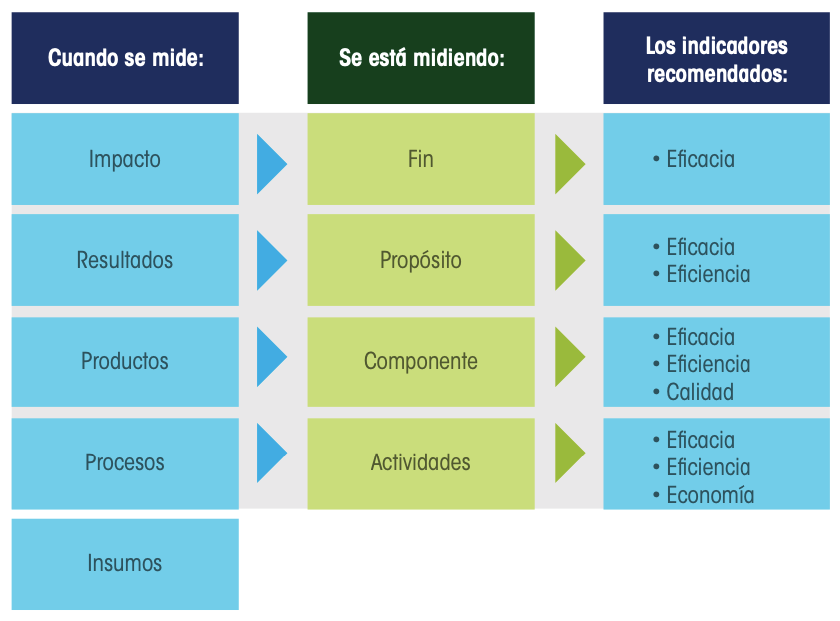
\includegraphics[width=0.7\linewidth]{Imagenes/figura_9} 

}

\caption{ Dimensiones sugeridas de los indicadores CONEVAL}\label{fig:figura9}
\end{figure}

Tomado de \citet{coneval2013manual}.

\begin{center}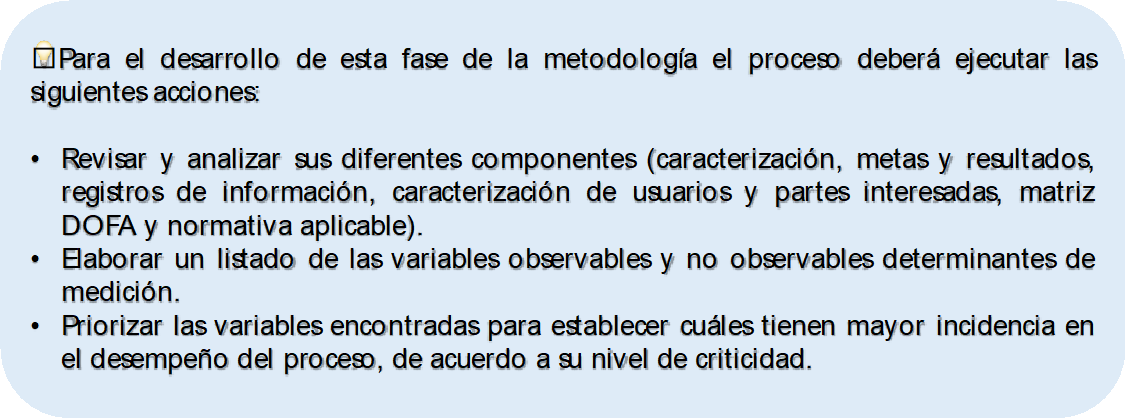
\includegraphics[width=0.7\linewidth]{Imagenes/texto} \end{center}

\hypertarget{diseuxf1o-de-la-mediciuxf3n-de-la-gestiuxf3n-de-los-procesos}{%
\section{Diseño de la medición de la gestión de los procesos}\label{diseuxf1o-de-la-mediciuxf3n-de-la-gestiuxf3n-de-los-procesos}}

La medición del desempeño de los procesos supone un esfuerzo institucional en la obtención de información de calidad que sea útil tanto para la toma de decisiones como para la rendición de cuentas a las partes interesadas, por lo que se deben establecer claramente cuales son los parámetros que permitan la caracterización de los indicadores de gestión en cuanto a su función, contexto y forma de uso. Para el caso de la UNAL se tomarán en cuenta los siguientes atributos:

\hypertarget{fuxf3rmula-del-indicador}{%
\subsection{Fórmula del indicador}\label{fuxf3rmula-del-indicador}}

Un aspecto importante al momento de diseñar un indicador consiste en establecer la relación matemática de las variables determinantes para su medición, con el fin de realizar el cálculo correspondiente y así obtener su valor cuantitativo. Para esto se requiere expresar el indicador a través de una ecuación en la que se utilizan símbolos para las expresiones aritméticas que denotan las operaciones matemáticas asociadas (\(\div\), \(\times\), \(+\), \(-\), \(()\)), en lugar de palabras (suma, resta, multiplicación, división, asociación, etc), así como identificadores (\(X\), \(Y\), \(Z\), etc.) para nombrar las variables determinantes de medición que la componen. Para ilustrar lo anterior, a continuación (\emph{Ver Figura \ref{fig:figura10}: Ejemplo fórmula de un indicador de gestión asociado a un proceso de la UNAL}) se muestra un ejemplo del cómo se debe escribir la fórmula asociada a un indicador de proceso:

\begin{figure}

{\centering 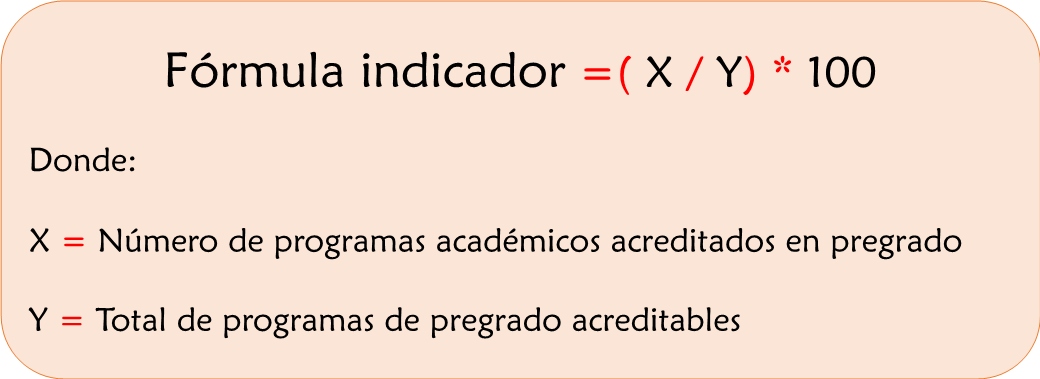
\includegraphics[width=0.7\linewidth]{Imagenes/figura_10} 

}

\caption{Ejemplo fórmula de indicador de gestión asociado a un proceso de la UNAL}\label{fig:figura10}
\end{figure}

\hypertarget{tipos-de-formulaciuxf3n-de-indicador}{%
\subsection{Tipos de formulación de indicador}\label{tipos-de-formulaciuxf3n-de-indicador}}

\begin{itemize}
\tightlist
\item
  \textbf{Frecuencia Absoluta (Cantidad):}
  Representa el número de veces que un valor \(x_i\) está en un conjunto de valores \((x_1, x_2, x_3, …, x_n)\). Se calcula a partir del recuento de la variable estudiada para ver el número de veces que aparece en el universo de datos:
\end{itemize}

\[
\sum_{i=1}^{k}x_i=x_1+x_2+\cdots+x_k=X
\]

\begin{figure}

{\centering 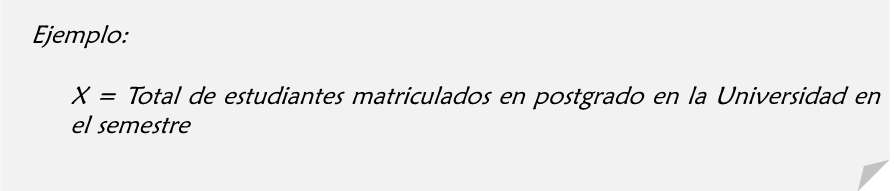
\includegraphics[width=0.7\linewidth]{Imagenes/texto_1} 

}

\caption{Ejemplo}\label{fig:unnamed-chunk-5}
\end{figure}

\begin{itemize}
\tightlist
\item
  \textbf{Frecuencia Relativa (Proporción):}
  De acuerdo con lo que establece \citet{coneval2013manual}, el porcentaje expresa un número como partes de cada cien. En términos de frecuencia relativa representa la proporcionalidad de una parte respecto al todo que generalmente esta dividido en \(n\) partes (100, 1000, etc.). Se calcula a partir del cociente entre dos variables con una misma unidad de medida en un periodo de tiempo determinado. A continuación, se muestra con un ejemplo la formulación de este tipo de indiciadores:
\end{itemize}

\begin{figure}

{\centering 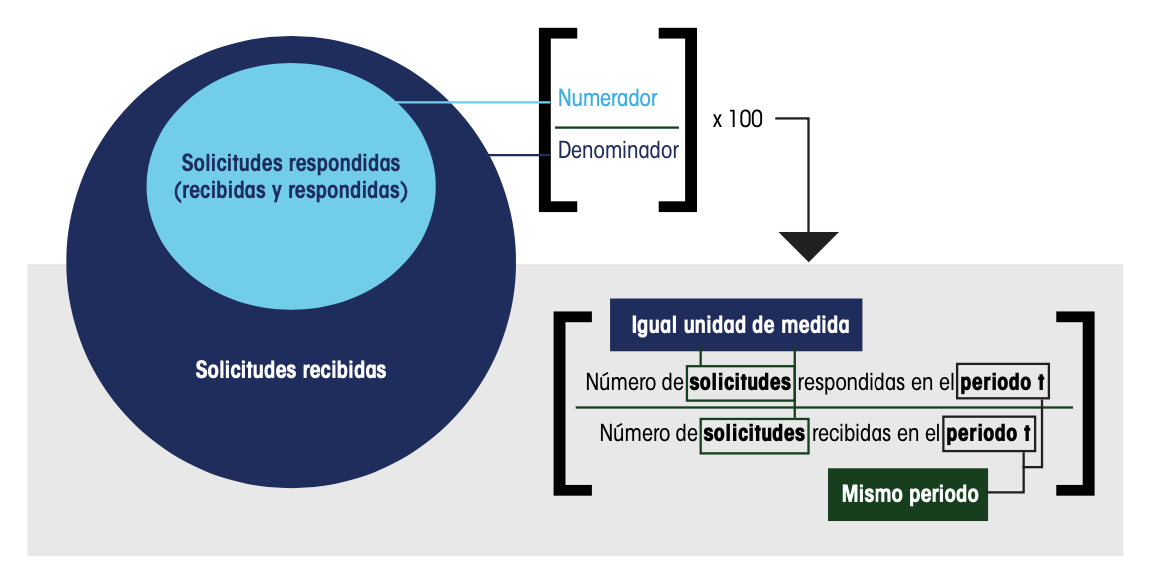
\includegraphics[width=0.9\linewidth]{Imagenes/figura_12} 

}

\caption{Ejemplo indicador formulado como porcentaje}\label{fig:unnamed-chunk-6}
\end{figure}

Tomado de \citet{coneval2013manual}.

\begin{center}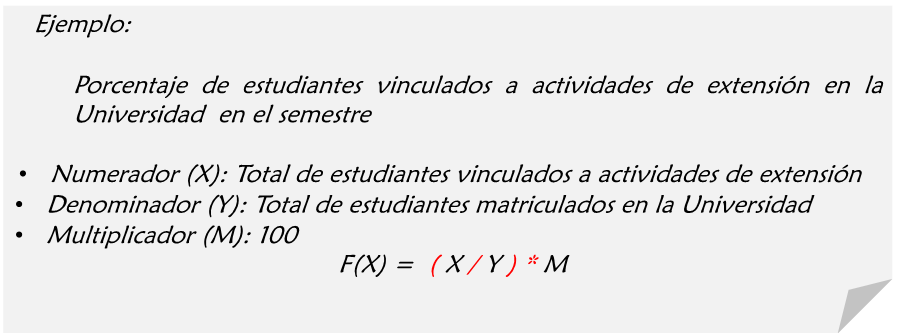
\includegraphics[width=0.7\linewidth]{Imagenes/texto_2} \end{center}

\begin{itemize}
\tightlist
\item
  \textbf{Tasa de variación:}
  Según \citet{coneval2013manual}, este tipo de medida expresa un cambio relativo en el tiempo a través del cociente de dos observaciones de una misma variable en diferentes periodos de tiempo (pasado \((t-k)\) y presente \((t)\)) para establecer si hubo un incremento o decremento de esta. Para su cálculo el periodo más reciente \((t)\) se coloca en el numerador mientras que el menos reciente se ubica en el denominador \((t-k)\).
\end{itemize}

\begin{figure}

{\centering 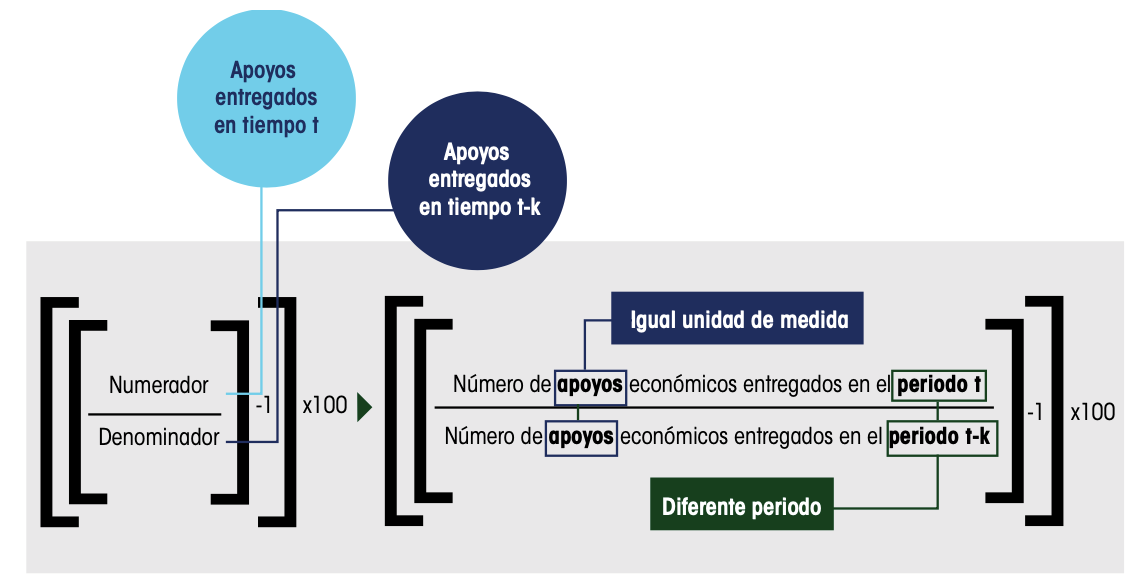
\includegraphics[width=0.9\linewidth]{Imagenes/figura_13} 

}

\caption{Ejemplo indicador formulado usando el método tasa de variación}\label{fig:unnamed-chunk-8}
\end{figure}

Tomado de \citet{coneval2013manual}.

\begin{itemize}
\tightlist
\item
  \textbf{Razón (Promedio):}
  Según \citet{coneval2013manual}, la define como el cociente entre dos variables en un periodo de tiempo determinado a través de la cual se expresa un tanto de unidades del numerador por cada unidad del denominador. El promedio es una particularidad de la razón en la que se tiene la suma finita de un conjunto de valores dividida entre el número de sumandos. Para su cálculo se tienen dos variables con diferentes unidades de medida, asociadas a un mismo periodo de tiempo.
\end{itemize}

\begin{figure}

{\centering 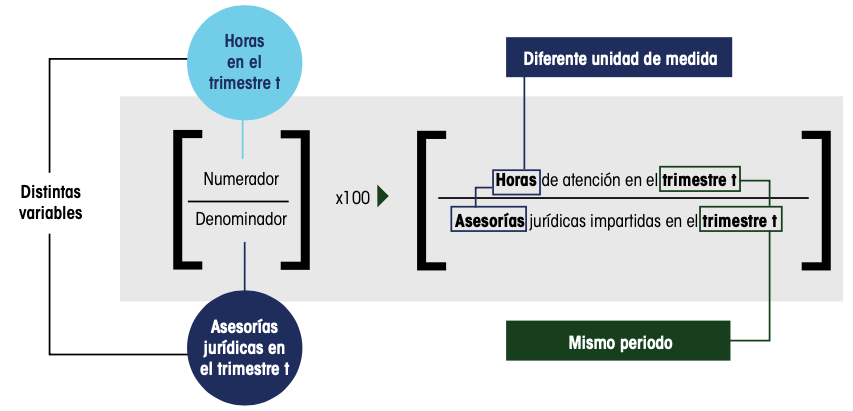
\includegraphics[width=0.9\linewidth]{Imagenes/figura_14} 

}

\caption{Ejemplo indicador formulado usando el método razón}\label{fig:unnamed-chunk-9}
\end{figure}

Tomado de \citet{coneval2013manual}.

\begin{center}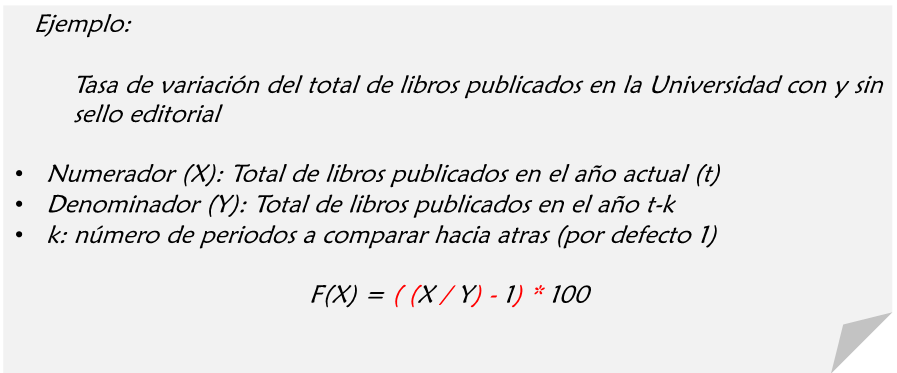
\includegraphics[width=0.7\linewidth]{Imagenes/texto_3} \end{center}

\begin{itemize}
\tightlist
\item
  \textbf{Índice:}
  Tal como especifica \citet{coneval2013manual}, se trata de una medida estadística que estudia las variaciones de una o más magnitudes en relación con el tiempo o el espacio.
\end{itemize}

Una vez definida la forma de cálculo del indicador es necesario establecer la direccionalidad de la medición, con lo cual se hace referencia a la dirección o rumbo del resultado obtenido pudiendo establecer si se cumple o no con lo esperado. Este sentido puede ser:

\begin{itemize}
\item
  \textbf{Ascendente:} Lo cual implica que la meta siempre es igual o mayor a la línea base o punto de referencia y que un buen desempeño se logra cuando el resultado de la medición del indicador aumenta de un periodo a otro.
\item
  \textbf{Descendente:} En este caso la meta se encuentra por debajo de la línea base y se espera que la medición del indicador vaya reduciéndose para mostrar el desempeño deseado.
\item
  \textbf{Regular:} Este sentido se da cuando el resultado esperado se debe mantener dentro de un determinado rango de desempeño (límite inferior y superior) y no cuenta con un valor puntual de meta.
\end{itemize}

\hypertarget{nombre-del-indicador}{%
\subsection{Nombre del indicador}\label{nombre-del-indicador}}

Al formular indicadores de gestión es importante tener en cuenta que su principal objetivo es medir los signos vitales de los procesos a partir de variables observables y no observables determinantes de medición, las cuales deben ser lo suficientemente relevantes para garantizar que de su monitoreo dependa la supervivencia institucional.

Por lo anterior, es recomendable nombrar el indicador de una manera clara, precisa y auto explicativa, de tal forma que logre distinguirse del universo de mediciones de la Universidad sin correr el riesgo de confundirse en una enorme cantidad de información. El nombre del indicador le dará una identidad propia por lo que debe resultar lo mas ilustrativo posible con relación a lo que se quiere medir, de manera que a continuación se sugiere una estructura de redacción compuesta por 5 elementos que lo caracterizan:

\begin{figure}

{\centering 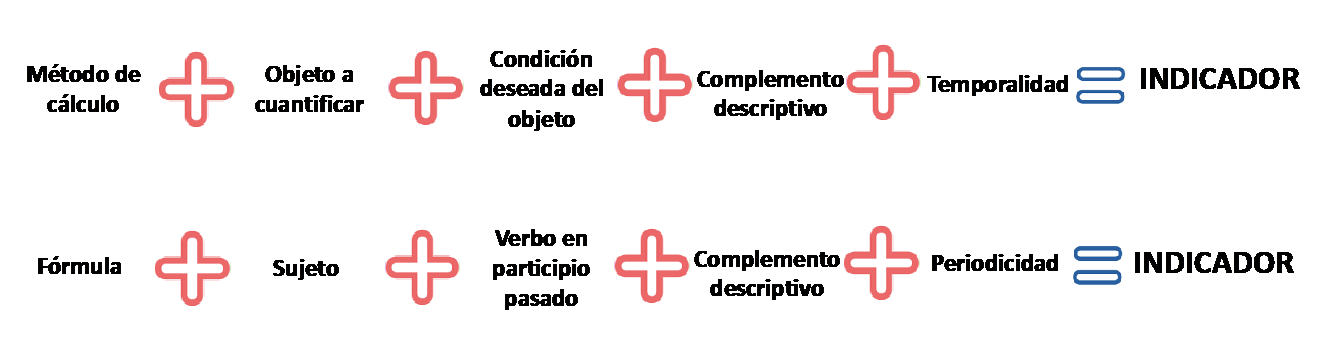
\includegraphics[width=0.9\linewidth]{Imagenes/figura_15} 

}

\caption{Fórmula para nombrar un indicador de gestión}\label{fig:unnamed-chunk-11}
\end{figure}

A partir de la aplicación de la fórmula propuesta se tiene los siguientes ejemplos de nombres para indicadores de gestión aplicables a los procesos de la Universidad:

\begin{center}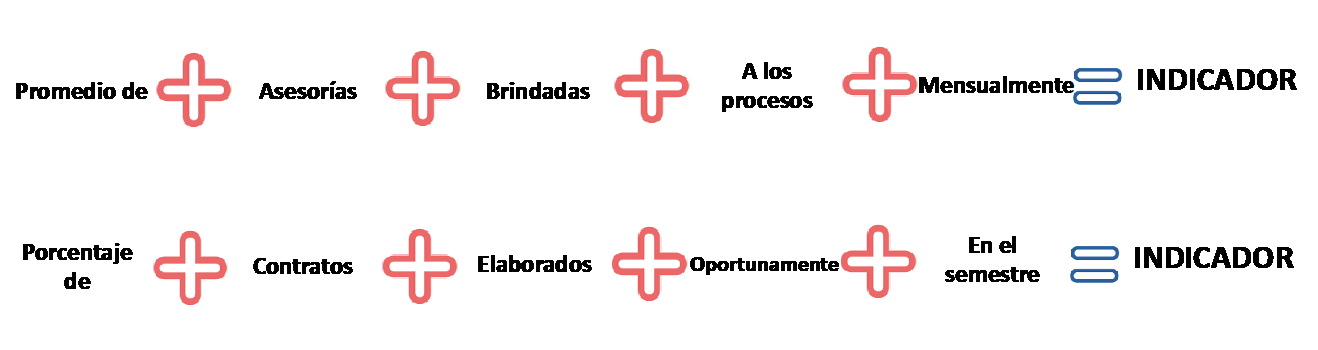
\includegraphics[width=0.9\linewidth]{Imagenes/figura_16} \end{center}

\begin{figure}

{\centering 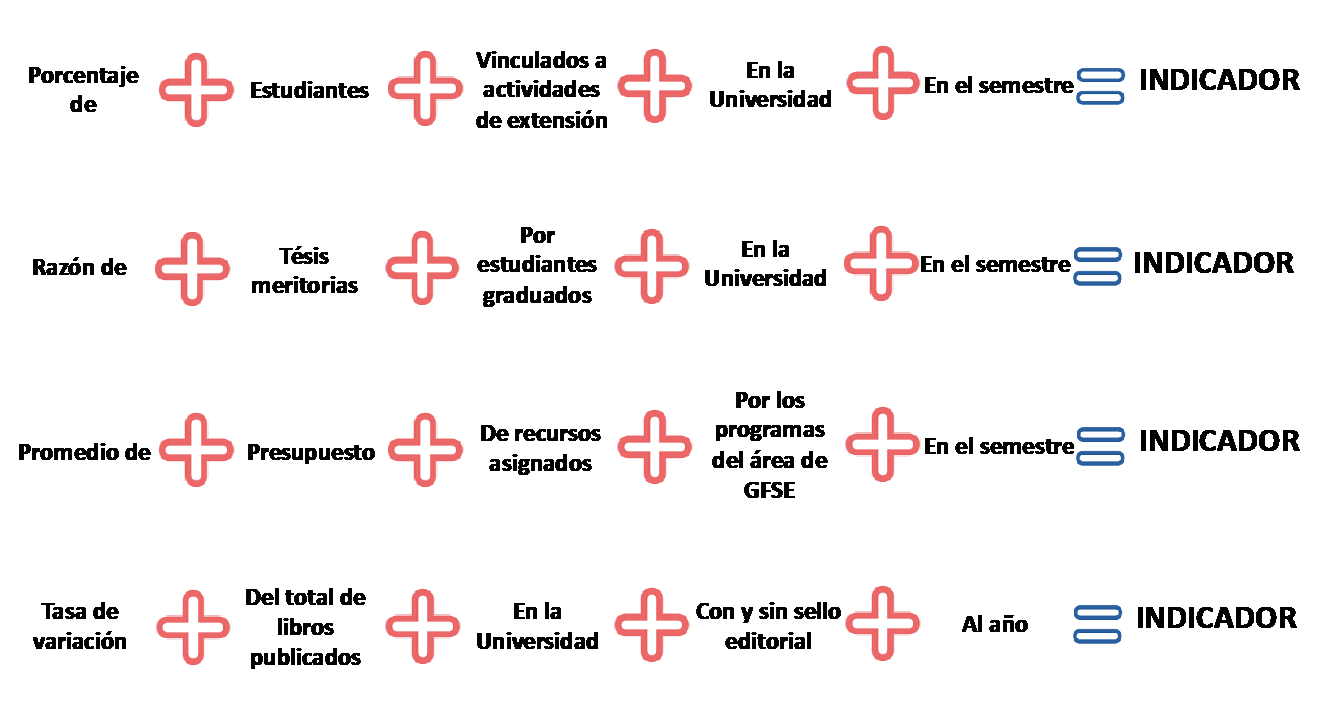
\includegraphics[width=0.9\linewidth]{Imagenes/figura_17} 

}

\caption{Ejemplos nombres indicadores de gestión aplicables en la UNAL}\label{fig:unnamed-chunk-13}
\end{figure}

Tomado de \citet{publica2015guia}.

Una vez se tenga claro el nombre del indicador se hará una descripción de este, en la que se justifique la importancia de su existencia en relación con el proceso que busca explicar sin que se incluyan los elementos mencionados en la anterior fórmula para no ser redundantes.

\hypertarget{fuentes-de-informaciuxf3n}{%
\subsection{Fuentes de información}\label{fuentes-de-informaciuxf3n}}

Continuando con el diseño de la medición se debe determinar el origen a partir del cual se obtendrán los datos puntuales que representan las variables asociadas al indicador, así como su localización y el método para su recolección. Para la Universidad se tiene una variedad de fuentes de información entre otros los que se destacan los siguientes tipos:

\begin{itemize}
\item
  Cifras oficiales: Estadísticas oficiales que se encuentran publicadas en los siguientes sitios web: \href{http://estadisticas.unal.edu.co/home/}{Estadísticas UNAL,}\href{http://estadisticas.unal.edu.co/menu-principal/cifras-sedes/bogota/}{Cifras UNAL sede Bogotá,}\href{http://estadisticas.unal.edu.co/menu-principal/cifras-sedes/bogota/,\%20http://estadisticas.unal.edu.co/menu-principal/cifras-sedes/medellin/}{Cifras UNAL sede Medellín,}\href{http://estadisticas.unal.edu.co/menu-principal/cifras-sedes/manizales/}{Cifras UNAL sede Manizales,}\href{http://estadisticas.unal.edu.co/menu-principal/cifras-sedes/palmira/,}{Cifras UNAL sede Palmira}\href{https://estadisticaun.github.io/BoletinOrinoquia/}{Cifras UNAL sede Orinoquía,}\href{http://gerencia.unal.edu.co/index.php?id=134}{Presupuesto UNAL,}\href{http://gerencia.unal.edu.co/index.php?id=147}{Memoria Financiera,}\href{http://cifrasvri.unal.edu.co/}{Indicadores - Vicerrectoría de Investigación.}
\item
  Registros de tipo administrativo que se pueden encontrar en sistemas de información institucionales (SARA, SIA, QUIPU, HERMES, SIBU, SINAB, SINSU, SoftExpert), bases de datos propias o en documentos tanto propios del proceso como de terceros bien sea en formatos, informes, archivos físicos o electrónicos.
\end{itemize}

Después de tener claridad sobre la ubicación de los datos fuente, así como de su disponibilidad para el uso, se debe definir el proceso de recolección de estos de acuerdo con la periodicidad de medición que se determine para cada indicador. Este proceso puede consistir en una consulta de un sistema de información o página web, la revisión de informes de gestión o de registros en medio físico o electrónico, el diligenciamiento de formularios o encuestas los cuales contengan los valores puntuales de las variables determinantes de medición o también se puede realizar por observación directa. Cabe aclarar que las fuentes de información no son las dependencias o procesos donde se generan los datos, ni los responsables de procesarla, consolidarla y presentarla.

El procesamiento incluye las operaciones necesarias para transformar los datos en información útil bien sea a través de procesos manuales como registro y clasificación o a través de procesos automáticos que incluyen filtrado, análisis, visualización y tabulación. En muchos casos se deberá fortalecer el registro administrativo de información bien sea en medios físicos o electrónicos para afinar las fuentes de datos antes de su procesamiento, porque es posibles que no existan los medios dispuestos para su captura.

\hypertarget{periodicidad-de-mediciuxf3n}{%
\subsection{Periodicidad de medición}\label{periodicidad-de-mediciuxf3n}}

No existe un estándar para establecer con qué periodicidad se requiere medir un indicador específico, lo importante es que dicha periodicidad tenga sentido para el proceso asociado, de ahí que la frecuencia seleccionada permita entregar información oportuna para la toma de decisiones y este relacionada con la disponibilidad (fuente de los datos) y accesibilidad de la información de entrada para su cálculo, así como el nivel de complejidad de la medición.

Si bien no se puede establecer el intervalo de tiempo ideal para el registro de los datos asociados a los indicadores de gestión, se recomienda que no sea tan estrecho (diario) que implique un desgaste institucional para los responsables designados, ni tan amplio (años) que impida generar alertas tempranas frente a cambios en el comportamiento del proceso. Al final la medición del indicador de gestión debe reflejar la realidad de aquello que busca explicar, en este caso, el cumplimiento del objetivo del proceso.

Es importante tomar conciencia que al establecer una frecuencia de medición se crea un compromiso por parte del responsable designado tanto para la actualización de la información como para la entrega oportuna de resultados a las partes interesadas, en pro de mostrar transparencia en la gestión de los procesos y como parte del ejercicio de rendición de cuentas permanente.

\hypertarget{luxednea-base}{%
\subsection{Línea base}\label{luxednea-base}}

Antes de establecer metas o rangos de desempeño es fundamental tener un punto de referencia en el momento cero de la medición del indicador con el que se pueda evidenciar el avance o retroceso de la gestión respecto al cumplimiento del objetivo del proceso asociado. En la mayoría de los casos se trata de un valor inicial del indicador, es decir el valor que toman las variables de cálculo en un periodo determinado, aunque también es posible calcularlo a partir del promedio de los valores que ha tomado en diferentes periodos en el pasado si se cuenta con suficientes datos históricos e incluso puede llegar a ser cero como en el caso de la ejecución de un proyecto.

La línea base se usa principalmente para fijar la meta de un indicador cuando no se tiene clara una apuesta a futuro, un estándar o valor de referencia (normativo o de la competencia), teniendo en cuenta que a partir de esta información se pueden hacer predicciones sobre el comportamiento del proceso a lo largo del tiempo. En este caso la meta podrá ser igual a la línea base o bien estar ubicada unos puntos por encima o por debajo dependiendo de la tendencia del indicador (ascendente, descendente o regular).

Los datos asociados a la línea base son útiles en la medida en que informan a los responsables de los procesos sobre las circunstancias actuales antes de proyectarse hacia el cumplimiento de metas, de esta manera se obtiene un aprendizaje de los niveles actuales y patrones de desempeño, resolviendo problemas de improvisación en la planeación. En otras palabras, la utilidad de la línea base consiste en conocer como estamos hoy para saber a donde queremos llegar mañana.

\hypertarget{establecimiento-de-rangos-de-desempeuxf1o-o-metas}{%
\subsection{Establecimiento de rangos de desempeño o metas}\label{establecimiento-de-rangos-de-desempeuxf1o-o-metas}}

La expresión concreta y cuantificable de los logros previstos en un horizonte de tiempo determinado con relación al cumplimiento del objetivo de un proceso, es lo que se denomina meta o rango de desempeño. En el caso de las entidades públicas algunas de estas metas están asociadas a obligaciones dadas por la norma o entes reguladores, mientras que otras dependen bien sea de apuestas a futuro propias, valores de referencia basados en resultados de competidores líderes o en análisis de datos históricos (línea base). Es importante aclarar que cuando el logro de los resultados está dado por una meta tendrá un valor puntual el cual podrá ser fijo o variable en el tiempo dependiendo de la estabilidad del proceso, mientras que cuando se trata de un rango de desempeño se deberá fijar un límite inferior y un límite superior entre los cuales se espera se mantengan las mediciones del indicador.

En cualquiera de los dos escenarios anteriormente expuestos se requiere que el nivel de desempeño a alcanzar puntual o rango, sea realista al tiempo que represente un desafío significativo para los responsables del despliegue del proceso, para no caer en extremos, de tener indicadores con cumplimientos por encima de la meta o indicadores que nunca pueden alcanzarla, esto garantizará que el valor fijado sea razonable.

Teniendo en cuenta esto, se recomienda que una vez el indicador haya mostrado un cumplimiento recurrente del desempeño esperado se revisen las metas o los rangos propuestos con el fin de ajustarlos y llevarlos a nuevos niveles más retadores para el proceso o si es el caso tomar la decisión de suspender su medición debido a que se ha cumplido su ciclo de vida (vencimiento). De igual forma se deben revisar las metas o rangos de desempeño cuando el indicador tenga un incumplimiento periódico, porque podría ser un síntoma de que los resultados previstos no son realistas y no es posible alcanzarlos con los recursos financieros, humanos, físicos y tecnológicos de los cuales dispone el proceso.

\hypertarget{hoja-de-vida-de-indicador-ficha-tuxe9cnica}{%
\subsection{Hoja de vida de indicador (Ficha técnica)}\label{hoja-de-vida-de-indicador-ficha-tuxe9cnica}}

Este instrumento brinda información valiosa relacionada con un indicador específico caracterizándolo de tal manera que cualquier parte interesada pueda conocer detalladamente los atributos que responden a las preguntas qué, quién, cuándo, dónde, para qué y cómo de la siguiente manera:

\begin{itemize}
\tightlist
\item
  \emph{Nombre:} Claro, sencillo y autoexplicativo.
\item
  \emph{Descripción:} Objetivo del indicador en relación con el proceso que pretende medir.
\item
  \emph{Proceso:} Nombre y código según los que establece el mapa de procesos vigente en la UNAL.
\item
  \emph{Nivel de aplicación:} Nivel Nacional, Sede, Facultad, Centro, Instituto y Laboratorios.
\item
  \emph{Cobertura del indicador:} Único (S/N).
\item
  \emph{Variables determinantes de desempeño:} Atributos a partir de los cuales se calcula el indicador. Hay que tener en cuenta que, en caso de usarse siglas para nombrar las variables, se debe hacer una nota explicativa para su descripción con el fin de que cualquier parte interesada comprenda a que hacen referencia.
\item
  \emph{Fuentes de información:} Ubicación de los datos que serán usados para las mediciones periódicas del indicador.
\item
  \emph{Tipo de formulación:} Forma de calculo del indicador (frecuencia absoluta, proporción, tasa de variación, razón, etc.).
\item
  \emph{Fórmula:} Expresión matemática usada para obtener el valor cuantitativo del indicador.
\item
  \emph{Unidad de medida:} Parámetro de referencia con el cual se determina la magnitud del indicador.
\item
  \emph{Periodicidad de medición:} Frecuencia con la que se recolectan los datos de entrada, se realiza el cálculo del indicador y se analizan los resultados.
\item
  \emph{Rango de desempeño o Meta:} Cantidad que se espera alcanzar en un periodo determinado o rango previsto dentro del que se espera mantenerse en un periodo de tiempo.
\item
  \emph{Responsable de medición:} Instancia y cargo del funcionario que debe registrar la información correspondiente a los valores cuantitativos del indicador con su análisis y acciones en caso de que se requiera.
\item
  \emph{Línea base (si aplica):} Información que permite describir el estado en que se encuentra el indicador en el momento cero de la medición.
\item
  \emph{Fecha de creación:} Corresponde al momento en que se formula y entra en vigencia el indicador.
\end{itemize}

La totalidad de la información asociada al indicador se podrá sistematizar de acuerdo con lo que se establece en el siguiente apartado.

\begin{center}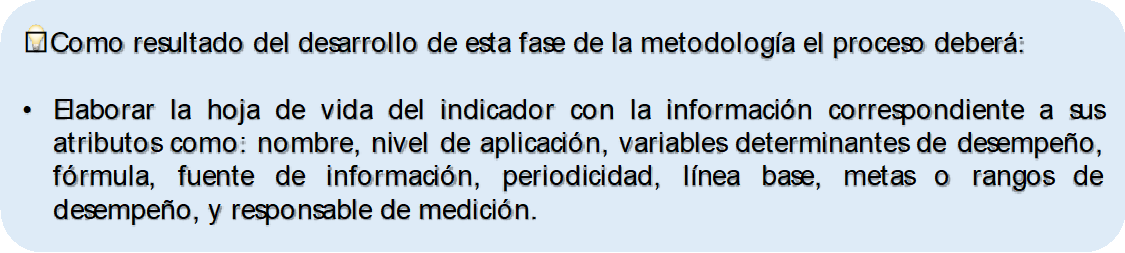
\includegraphics[width=0.8\linewidth]{Imagenes/texto_5} \end{center}

\hypertarget{sistematizaciuxf3n-de-los-indicadores-de-gestiuxf3n}{%
\chapter{Sistematización de los indicadores de gestión}\label{sistematizaciuxf3n-de-los-indicadores-de-gestiuxf3n}}

La Universidad Nacional cuenta con un software de tipo modular para la gestión integrada de la información asociada al Sistema Integrado de Gestión Académica, Administrativa y Ambiental SIGA, en el que se incluye el módulo de \emph{``Desempeño''}, con el cual se administran y monitorean los indicadores de gestión asociados a los procesos, contemplando a grandes rasgos las siguientes actividades:

\begin{figure}

{\centering 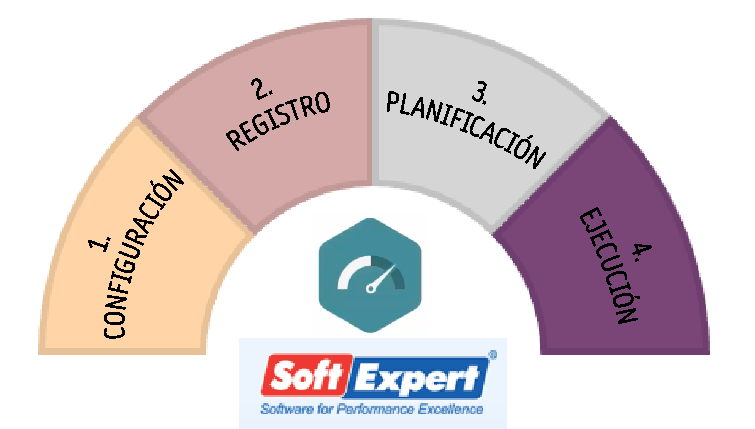
\includegraphics[width=0.7\linewidth]{Imagenes/figura_17a} 

}

\caption{Fases para la sistematización de indicadores de gestión módulo *“Desempeño”*}\label{fig:unnamed-chunk-15}
\end{figure}

\begin{enumerate}
\def\labelenumi{\arabic{enumi}.}
\item
  \textbf{Configuración inicial} del módulo de acuerdo a la metodología adoptada por la UNAL que incluyen la programación de mediciones periódicas de las baterías de indicadores, registro de metadatos (atributos asociados a los indicadores), niveles de responsabilidad (grupos de usuarios responsables de ejercer diferentes funciones), configuración de eventos (problema, incidente, plan de acción) a partir de reglas predefinidas, rango de desempeño, visualización gráfica de la medición del indicador, jerarquía de indicadores, unidades de medida, perfil de visualización (estructura de la batería de indicadores, historial del resultado del indicador, detalles del indicador y listado de indicadores), tipos de análisis gráficos.
\item
  \textbf{Registro de información} que será utilizada en el momento de la planificación, ejecución y gestión de las baterías de indicadores como elementos institucionales (perspectivas, objetivos, áreas, sedes, procesos, visión, misión y valores, entre otros), factores críticos de éxito (variables determinantes de desempeño), indicadores de gestión, matriz de decisión, matriz DOFA, modelo de las baterías de indicadores.
\item
  \textbf{Planificación de la estructura de las baterías de indicadores} asociando elementos institucionales (perspectivas, objetivos, procesos), matriz de decisión, matriz DOFA, documentos referentes, plan de acción, controles, riesgos, factores críticos de éxitos (variables determinantes de desempeño), indicadores de gestión, fórmulas de cálculo, metas, responsabilidades en cada nivel de aplicación, plazos de reporte de mediciones, definición de análisis gráfico comparativo con otros periodos de medición o con otros indicadores.
\item
  \textbf{Ejecución de mediciones periódicas} programadas de cada uno de los indicadores de manera manual o automática y análisis cualitativo de resultados.
\end{enumerate}

Para profundizar en el funcionamiento del módulo de ``Desempeño'' se recomienda consultar el manual de usuario del SoftExpert© con las instrucciones detallas para ejecutar las acciones correspondientes a cada una de las etapas mencionadas.

\begin{figure}

{\centering 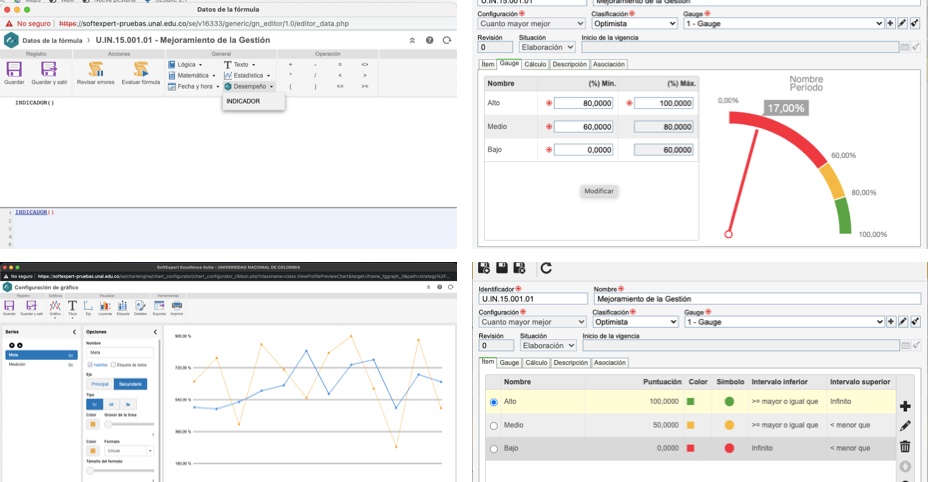
\includegraphics[width=1\linewidth]{Imagenes/figura_18} 

}

\caption{Pantallazos configuración módulo de *“Desempeño”* SoftExpert}\label{fig:unnamed-chunk-16}
\end{figure}

Es importante mencionar la ventaja que ofrece la sistematización de los indicadores de gestión en lo que respecta a la posibilidad de tener en un repositorio único que almacene la totalidad de los datos asociados al desempeño de los procesos, permitiendo su reutilización para diferentes fines, evitando la duplicidad de información y el desgaste institucional para la presentación de resultados a las partes interesadas.

Sin embargo y a pesar que el SIGA promueva la administración de la información a través de una herramienta única a nivel institucional, es importante mencionar que en la práctica los procesos pueden gestionar sus indicadores de desempeño a través de sistemas de información propios, siempre y cuando cumplan con los lineamientos dados en la presente guía y brinden facilidades de acceso para la consulta por parte de los diferentes usuarios de acuerdo a su nivel de confidencialidad, así como para su consolidación a nivel institucional como insumo en la elaboración de informes de resultados.

\begin{center}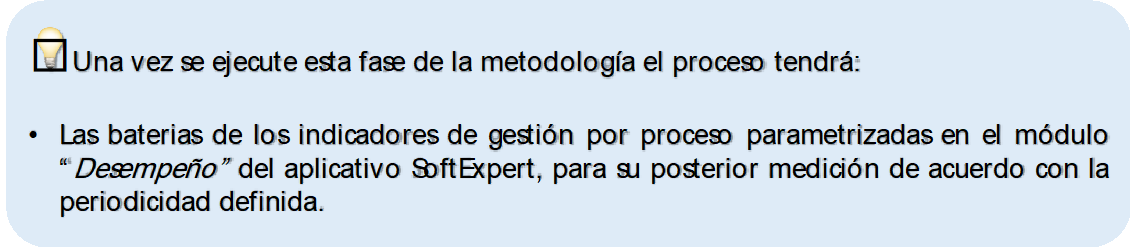
\includegraphics[width=0.8\linewidth]{Imagenes/texto_6} \end{center}

\hypertarget{mediciuxf3n-de-los-indicadores-de-gestiuxf3n-de-acuerdo-con-su-periodicidad}{%
\chapter{Medición de los indicadores de gestión de acuerdo con su periodicidad}\label{mediciuxf3n-de-los-indicadores-de-gestiuxf3n-de-acuerdo-con-su-periodicidad}}

Un indicador de gestión es útil una vez se ha medido, pues sólo hasta ese momento se puede establecer si la información resultante describe realmente la situación actual en que se encuentra un proceso a partir del comportamiento de sus variables determinantes.

Para realizar esta medición es necesario que el responsable asignado acuda a las fuentes de información y realice las consultas de los datos correspondientes de acuerdo con la periodicidad previamente definida, para su posterior registro en el módulo de ``desempeño'' del aplicativo SoftExpert con el usuario y clave asignado, de tal manera que se realicen los cálculos del valor final que tomará cada indicador de gestión en particular. El ingreso de la información deberá hacerse siguiendo las instrucciones dadas en el manual de usuario del mencionado módulo a través bien sea de las tareas pendientes asignadas o del menú \emph{``General''} en el submenú \emph{``Ejecución''}. (\emph{Ver Figura \ref{fig:figura19}. Pantallazos medición de indicadores módulo ``Desempeño'' SoftExpert©})

\begin{figure}

{\centering 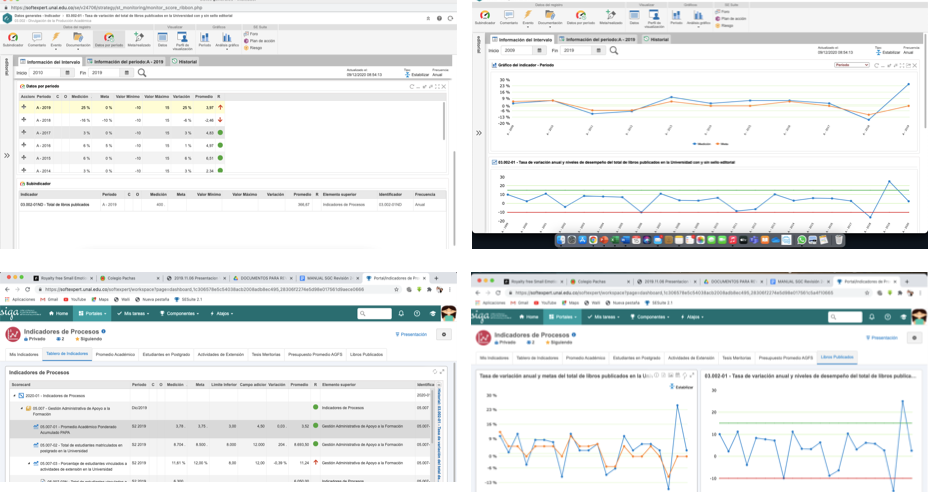
\includegraphics[width=0.8\linewidth]{Imagenes/figura_19} 

}

\caption{Pantallazos medición de indicadores módulo de “Desempeño” SoftExpert©}\label{fig:figura19}
\end{figure}

\begin{center}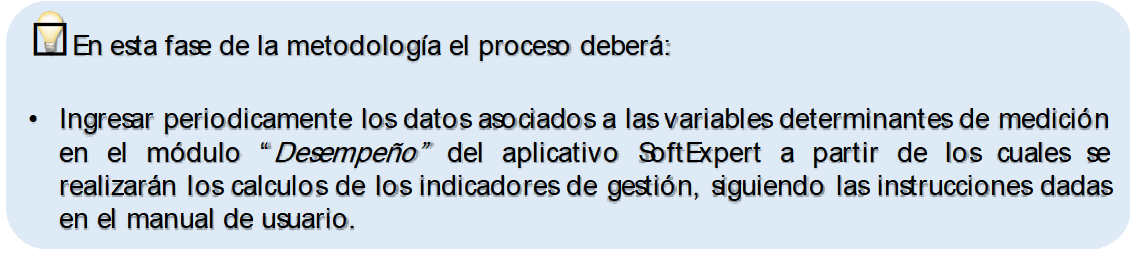
\includegraphics[width=0.8\linewidth]{Imagenes/texto_7} \end{center}

\hypertarget{anuxe1lisis-de-resultados-de-mediciuxf3n-y-toma-de-decisiones}{%
\chapter{Análisis de resultados de medición y toma de decisiones}\label{anuxe1lisis-de-resultados-de-mediciuxf3n-y-toma-de-decisiones}}

Para la interpretación de los resultados obtenidos a partir de la recolección y el procesamiento de los datos asociados a los indicadores, estos deben ubicarse en el contexto del proceso al que pertenecen y de esta manera poder inferir específicamente sobre su comportamiento. Este tipo de análisis tiene que ver con la identificación de la relación causa efecto en cuanto a cómo se alcanzaron los resultados y establecer que tan lejos o cerca se está del logro de las metas o los rangos de desempeño propuestos. Por lo anterior es conveniente iniciar la argumentación respondiendo las siguientes preguntas:

\begin{itemize}
\tightlist
\item
  ¿El indicador cumplió/incumplió la meta o el rango de desempeño en el periodo de medición?
\item
  ¿Cuáles fueron las causas del cumplimiento/incumplimiento de la meta o el rango de desempeño en el periodo de medición?
\item
  ¿Qué acciones se deben tomar para mantener o alcanzar la meta o rango de desempeño propuesto?
\end{itemize}

De igual forma se recomienda presentar los resultados de medición de los indicadores haciendo uso de diferentes herramientas estadísticas, que permitan mostrar la distribución de los datos de acuerdo con características que sean de interés para los procesos. Como referente en este tema se tiene el informe técnico \emph{ISO/TR 10017 Orientación sobre las técnicas estadísticas para la Norma ISO 9001:2000} y la \emph{U.GU.SIGA.001 Guía Básica de Mejora V4} en el que se destacan herramientas de tipo descriptivo principalmente por su facilidad para el despliegue de los datos de manera simple a través de una variedad de métodos gráficos entre los que se encuentran:

\begin{itemize}
\item
  El gráfico lineal (tendencia), compuesto por una serie de datos representados por puntos unidos por segmentos lineales, el cual se utiliza para ver el comportamiento de variables cuantitativas en el transcurso del tiempo.
  • El diagrama de dispersión, en el que se evalúa la relación entre dos variables a través de una representación gráfica de una de ellas en el eje X respecto a la otra en el eje Y.
\item
  El histograma, como una representación de variables cualitativas en forma de barras rectangulares cuya altura es proporcional a la frecuencia de los valores de la variable estudiada.
\item
  El diagrama circular (torta), que representa la proporción de elementos de cada uno de los valores de una variable. En donde cada porción representa cada valor que toma la variable.
\item
  El diagrama de Pareto, como representación de cada una de las categorías de las variables cuantitativas a través de un rectángulo que es proporcional a su frecuencia, de manera que se ordenan los datos por su frecuencia relativa o absoluta.
\end{itemize}

Por otra parte la U.GU.SIGA. 001 Guía Básica de Mejora V4 menciona las técnicas para la resolución de problemas que se enuncian a continuación, las cuales pueden ser de utilidad para enriquecer el análisis de resultados y la toma de decisiones:

\begin{itemize}
\item
  Diagrama de causa -- efecto (Espina de pescado), es una representación gráfica que permite identificar en este caso las causas de cumplimiento o incumplimiento de la meta de un indicador, clasificándolas en 5 categorías 5M (Método, Mano de obra, Maquinaria, Materiales y Medio ambiente).
\item
  Cinco porque, se centra en el análisis de las causas del resultado de la medición del indicador a través de 5 preguntas sucesivas del por qué ocurre la situación concreta hasta llegar a la raíz que la origina.
\end{itemize}

Una vez se realice el análisis de resultados se tendrá acceso a información confiable y oportuna para hacer uso de ella en el proceso de toma de decisiones, es por esta razón que los indicadores de gestión pueden considerarse elementos que dan cuenta del comportamiento de las variables críticas de los procesos de tal manera que se pueda eliminar, incluir o ajustar aquello que sea más o menos útil para el logro de sus objetivos. Lo anterior parece simple, pero en la práctica para que exista un discernimiento organizacional efectivo es necesario tener en cuenta los siguientes aspectos:

\begin{itemize}
\item
  Garantizar que los datos y la información de entrada para el cálculo de los indicadores de gestión son suficientemente precisos y fiables. Los datos se deben obtener de fuentes de información en lo posible oficiales o documentos y registros verificables.
\item
  Permitir el acceso a los datos a las partes interesadas del proceso. La Universidad debe establecer los medios adecuados para el almacenamiento y la consulta de la información a través de los canales institucionales oportunos (sistemas de información o informes de resultados).
\item
  Analizar los datos y la información con una metodología adecuada. Es necesario que se realice el seguimiento y análisis de los datos de una manera iterativa y con una frecuencia establecida de forma que se puedan separar aquellos que son relevantes de los que no lo son. También, se debe establecer rangos de desempeño para cada uno de los indicadores de gestión definidos en el sistema de medición y en el caso de superarlos o no alcanzarlos, formular acciones preventivas o correctivas según corresponda.
\item
  Implementar acciones basadas en el análisis objetivo de la información disponible, en equilibrio con la experiencia y conocimiento de los responsables de la toma de decisiones. En otras palabras, cualquier actividad planteada debe tener un análisis de causas asociado.
\item
  El resultado de la ejecución de las acciones debe llevar a fortalecer la estrategia institucional, el logro de las metas propuestas, identificación y resolución de problemas y oportunidades, a un mayor entendimiento de los procesos y al igual que al mejoramiento de los controles institucionales.
\end{itemize}

\begin{center}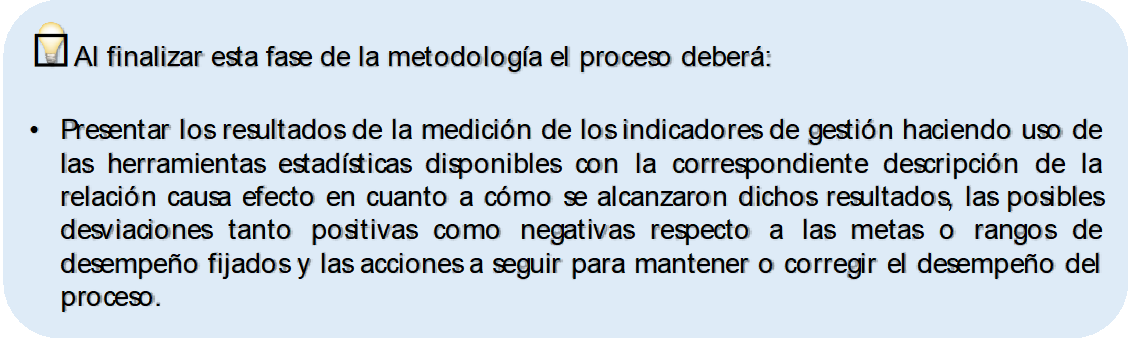
\includegraphics[width=0.8\linewidth]{Imagenes/texto_8} \end{center}

\hypertarget{presentaciuxf3n-de-informaciuxf3n-a-partes-interesadas}{%
\chapter{Presentación de información a partes interesadas}\label{presentaciuxf3n-de-informaciuxf3n-a-partes-interesadas}}

Una parte fundamental de la cuantificación, medición y seguimiento a la gestión de los procesos consiste en la presentación de resultados a las partes interesadas de manera estructurada, bien sea para demostrar conformidad frente a los requisitos del sistema de gestión de calidad institucional y la normativa aplicable o como mecanismo de transparencia y rendición de cuentas puesto que se trata de una obligación y responsabilidad de cualquier entidad pública. En este sentido el informe de seguimiento a los indicadores de gestión debe cumplir con características como impacto visual de forma relacionando el orden cronológico y secuencial de la presentación de la información, así como en el uso de recursos gráficos, también debe tener profundidad en el contenido a través de una clara exposición de ideas, contemplando siempre el público al que va dirigido de tal manera que incentive su lectura en la medida que sea comprensible y consistente. Para la redacción del informe se puede emplear la estructura clásica que abarca una introducción, nudo y desenlace con los elementos que se muestran a continuación:

\begin{itemize}
\item
  En la \textbf{introducción} se presenta un texto breve en el que se aclara el objetivo del informe de tal manera que se pueda entender la totalidad del documento.
\item
  En el \textbf{nudo} se detallan las realidades tanto positivas como negativas que han surgido como consecuencia de la medición de los indicadores de gestión. Esta parte del informe se compone de un texto explicativo alternado con gráficos como diagramas o infografías (Ver Figura \ref{fig:figura20}: Ejemplos infografías para la presentación de resultados) y tablas con datos fuente. Es importante tener presente que la extensión, profundidad y complejidad del análisis de resultados dependerá del tipo de redacción y la magnitud de la información base, sin embargo, es recomendable usar un lenguaje claro y sencillo y asegurar que se determinan las causas de dichos resultados y las repercusiones esperadas en los procesos.
\item
  Y finalmente en el \textbf{desenlace} se formulan las reflexiones, conclusiones (juicios de valor) y acciones a tomar (mantener, prevenir o corregir) a partir de la información resultante.
\end{itemize}

Adicional a los elementos anteriores, el informe debe incluir la fecha y el responsable de su elaboración además de la imagen institucional de acuerdo con los formatos para la presentación de informes oficiales establecidos a nivel institucional.

\begin{figure}

{\centering 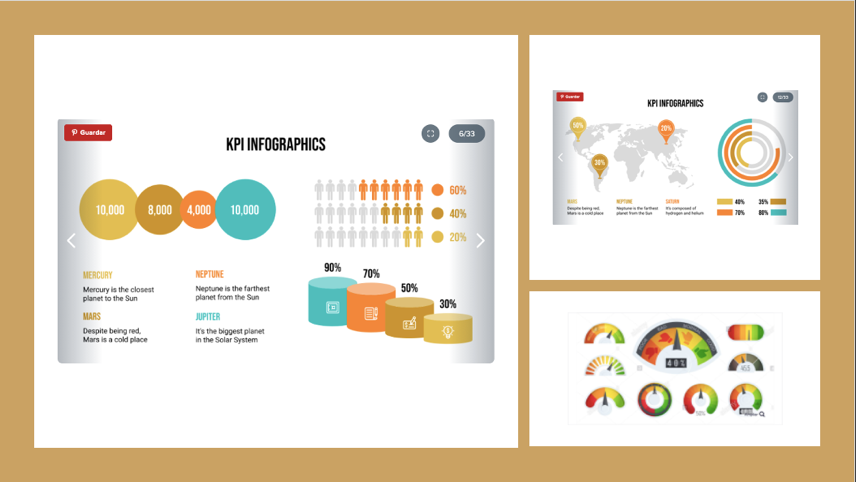
\includegraphics[width=0.8\linewidth]{Imagenes/figura_20} 

}

\caption{Ejemplos infografías para la presentación de resultados}\label{fig:figura20}
\end{figure}

Es importante mencionar que cada informe debe recoger, tanto los resultados obtenidos de las mediciones de los indicadores de desempeño, ordenados y estructurados utilizando el método que mejor se adapte a las necesidades de cada proceso (técnicas estadísticas), como la descripción cualitativa de las causas que originen bien sea el cumplimiento de las metas o rangos de desempeño o las desviaciones tanto positivas como negativas según el caso, así como las medidas tomadas para mantener o corregir estos resultados y regular la operación del proceso. De esta manera se podrá informar a las partes interesadas lo que sucede en la realidad del proceso y el por qué sucede esto.

Adicional a los informes, los procesos deben garantizar que los resultados de las mediciones de sus indicadores de gestión son accesibles para sus partes interesadas bien sea a través de la publicación de sus baterías en el enlace de \emph{Transparencia y acceso a la información}, en las páginas web oficiales, o con la emisión de infografías vía postmaster y la promoción de su consulta en el módulo \emph{``Desempeño''} del aplicativo SoftExpert, por mencionar algunos ejemplos.

\hypertarget{monitoreo-del-sistema-de-indicadores-de-gestiuxf3n-de-los-procesos-unal}{%
\section{Monitoreo del sistema de indicadores de gestión de los procesos UNAL}\label{monitoreo-del-sistema-de-indicadores-de-gestiuxf3n-de-los-procesos-unal}}

El monitoreo del sistema de indicadores consiste en un método de autoevaluación en el que los procesos deberán realizar una revisión periódica, al menos dos veces al año (puede ser semestral), de cada indicador de desempeño, así como de las mediciones, del análisis de resultados y las acciones derivadas de este, asegurando su validez y calidad y consignando sus apreciaciones en las plantillas que establezca el SIGA. Se debe tener en cuenta que uno de estos monitoreos podrá corresponder con el reporte que se presenta en la revisión por la dirección del SGC.

\begin{center}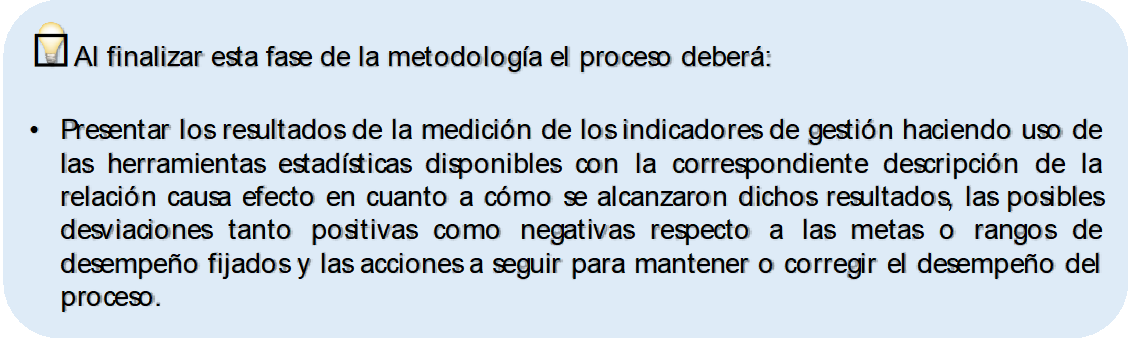
\includegraphics[width=1\linewidth]{Imagenes/texto_9} \end{center}

\hypertarget{diseuxf1o-de-la-bateruxeda-tablero-de-control-de-indicadores-de-gestiuxf3n-por-proceso}{%
\chapter{Diseño de la batería (Tablero de control) de indicadores de gestión por proceso}\label{diseuxf1o-de-la-bateruxeda-tablero-de-control-de-indicadores-de-gestiuxf3n-por-proceso}}

Para garantizar que la medición de los indicadores refleje la gestión de la totalidad de los procesos aplicables en la UNAL es necesario establecer sus diferentes niveles de aplicación teniendo en cuenta los contextos particulares (nivel nacional, sedes andinas y de presencia nacional, centros, facultades, institutos y laboratorios) en los que se despliegan sus objetivos. En efecto, el hecho de contar con múltiples indicadores asociados a un mismo proceso requiere de una estructura y forma de presentación que facilite su análisis sin que pierdan relevancia o muestren comportamientos disfuncionales asociados a un exceso de información. Por lo que, en la figura \ref{fig:figura21} se propone el modelo institucional para la adopción de una batería de indicadores por proceso concebida como una herramienta que permite su gestión de acuerdo con los roles y responsabilidades definidos y su consolidación a nivel institucional, buscando que los indicadores que la conforman se complementen entre si y puedan ofrecer una visión completa respecto al cumplimiento de sus objetivos y metas.

\begin{figure}

{\centering 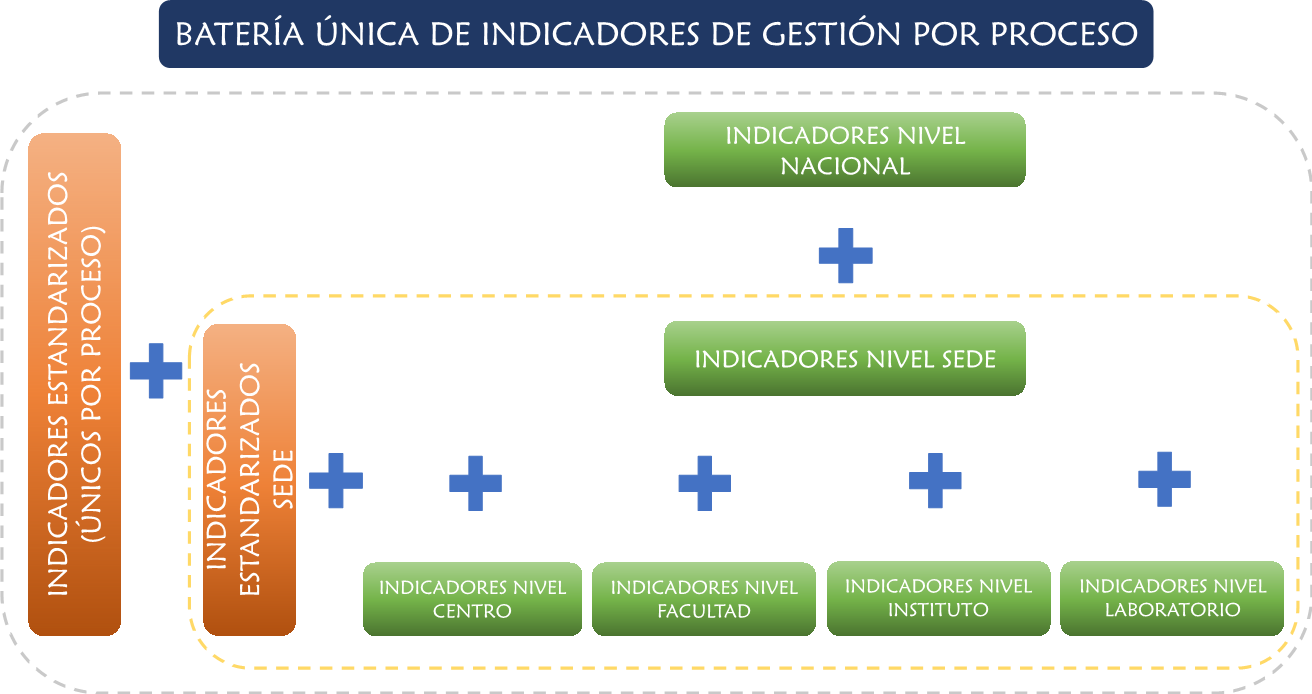
\includegraphics[width=0.8\linewidth]{Imagenes/figura_21} 

}

\caption{Estructura baterías de indicadores de gestión por proceso UNAL}\label{fig:figura21}
\end{figure}

Con base en lo anterior, se tiene los siguientes tipos de indicadores de gestión aplicables en los procesos de la UNAL:

\begin{itemize}
\item
  \textbf{Indicadores estandarizados (únicos):} Esta categoría agrupa indicadores cuyos atributos (nombre, descripción, fórmula, periodicidad, meta, línea base, etc\ldots) son idénticos en todos los niveles de aplicación (nacional, sedes andinas y de presencia, facultades, centros, institutos y laboratorios) y solo varían las mediciones puntuales que se ejecuten en cada uno de ellos. También se pueden enmarcar en esta categoría los indicadores que se calculan de manera consolidada a nivel institucional y entregan un solo dato para toda la universidad.
\item
  \textbf{Indicadores nivel nacional:}Consisten en indicadores que son formulados y medidos exclusivamente en los procesos en el nivel nacional y no tienen cobertura en los niveles inferiores.
\item
  \textbf{Indicadores estandarizados sede:} Contemplan formulaciones y mediciones que abarcan los procesos en los niveles central, facultades, centros, institutos y laboratorios para una o varias sedes.
\item
  \textbf{Indicadores nivel sede:} Abarcan formulación y mediciones en los procesos de una o varias sedes a nivel central sin llegar a las facultades, centros, institutos y laboratorios.
\item
  \textbf{Indicadores nivel centro / facultad / instituto / laboratorio:} Son medidas que determinan la gestión de los procesos puntualmente en facultades, centros, institutos y laboratorios sin llegar a aplicarse en los niveles superiores. Cuentan con variables determinantes de medición, fórmulas y metas propias.
\end{itemize}

\hypertarget{esquema-de-comunicaciuxf3n-frente-a-la-definiciuxf3n-de-indicadores-de-gestiuxf3n}{%
\chapter{Esquema de comunicación frente a la definición de indicadores de gestión}\label{esquema-de-comunicaciuxf3n-frente-a-la-definiciuxf3n-de-indicadores-de-gestiuxf3n}}

De acuerdo con la definición de los roles y responsabilidades (\emph{Ver Tabla \ref{tab:tabla2}: Roles en la cuantificación, medición y seguimiento a la gestión de los procesos en la UNAL}) para el desarrollo de las diferentes actividades asociadas al componente de cuantificación, medición y seguimiento a la gestión de los procesos se determinó una estructura de flujo de comunicación (\emph{Ver Figura \ref{fig:figura22}: Estructura flujo de comunicación componente medición, cuantificación y seguimiento UNAL}), la cual permite visualizar el grado de participación de los diferentes actores y enmarcar acuerdos y compromisos que puedan dar claridad sobre los grados de responsabilidad de cada uno de ellos frente a la información desde su recolección, pasando por su producción y análisis hasta su difusión. Esto contribuirá significativamente en la calidad y oportunidad de la toma de decisiones y el mejoramiento de los procesos.

\begin{figure}

{\centering 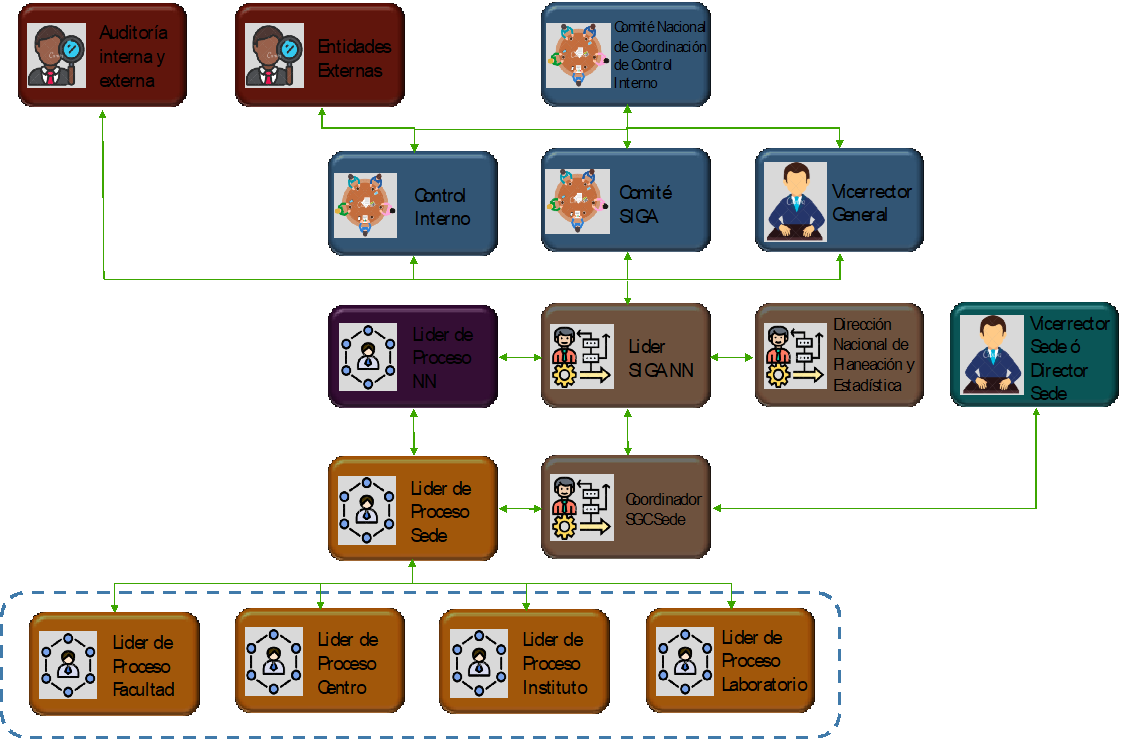
\includegraphics[width=0.8\linewidth]{Imagenes/figura_22} 

}

\caption{Estructura flujo de comunicación componente medición, cuantificación y seguimiento UNAL}\label{fig:figura22}
\end{figure}

Esta estructura debe aplicarse en las diferentes etapas en las que se desarrolla la metodología para la definición de los indicadores de gestión garantizando tanto su apropiación como su correcta puesta en marcha en todos los niveles en los que se despliegan los procesos de la UNAL. El flujo de comunicación se da en sentido descendente desde el líder de los procesos en el nivel nacional hacia los líderes en niveles más bajos (Sede -- Facultad, Centro, Instituto, Laboratorio), en concordancia con el nivel de aplicación definido en su correspondiente caracterización, esto quiere decir que si un proceso no tiene aplicación en el nivel nacional este se obviará en la batería de indicadores, por ejemplo. De igual forma se debe tener en cuenta el uso, en lo posible, de redes formales de comunicación para coordinar las tareas derivadas del despliegue del componente de cuantificación, medición y seguimiento a la gestión, de tal manera que se garantice la calidad y oportunidad en la entrega de la información de todos los niveles para su recopilación institucional.

\hypertarget{gestiuxf3n-de-cambio}{%
\chapter{Gestión de cambio}\label{gestiuxf3n-de-cambio}}

\begin{itemize}
\item
  \textbf{¿Qué cambios se van a introducir?} En el marco del proyecto BPUN 358 2019 -- 2021 \emph{``Transformación de la cultura organizacional desde el enfoque de generación de valor''}, Meta 5.1 Elaborar un documento con la metodología para la cuantificación, medición y seguimiento de la gestión de los procesos, la UNAL se ha propuesto rediseñar la guía para la formulación de indicadores de gestión, incorporando herramientas que faciliten la apropiación de los diferentes conceptos asociados a la medición del desempeño de los procesos, al tiempo que los líderes y gestores puedan poner en práctica el paso a paso para su correcta puesta en marcha.
\item
  \textbf{¿Para qué hacer estos cambios?} La mejora continua es un enfoque que debe incorporarse en la operación de cualquier entidad dispuesta a adaptarse a la realidad de su contexto para garantizar su supervivencia. En este sentido los cambios metodológicos que se den en cuanto a la forma en que se mide el desempeño de sus procesos deben orientarse a la aplicación de herramientas claras y sencillas que contribuyan a la toma de decisiones sobre una base solida de información confiable y oportuna y no solo limitarse al cumplimiento de compromisos normativos o dados por entes de certificación.
\item
  \textbf{¿Qué beneficios traerán los cambios propuestos?} La aplicación de una metodología rediseñada para la medición, cuantificación y seguimiento a la gestión de los procesos aportará a la rendición de cuentas promoviendo la transparencia en la gestión institucional, en la medida en que se pueda evidenciar el desempeño de los procesos a través de indicadores que estructuren la información para determinar de manera objetiva si efectivamente se están cumplimiento los objetivos y metas trazados.
\end{itemize}

El cambio metodológico busca aportar significado, relevancia y entendimiento a la gestión de los procesos de la UNAL porque permite describir el estado real en que se encuentran en determinado momento, al tiempo que añade un juicio de valor, lo mas objetivo posible, sobre la adecuación de su desempeño para orientar la posterior toma de decisiones y finalmente comunicar a las diversas partes interesadas estos resultados.

\hypertarget{anexos}{%
\chapter{Anexos}\label{anexos}}

\hypertarget{anexo-1-lineamientos-para-la-priorizaciuxf3n-de-variables-determinantes-de-mediciuxf3n}{%
\subsection{Anexo 1: Lineamientos para la priorización de variables determinantes de medición}\label{anexo-1-lineamientos-para-la-priorizaciuxf3n-de-variables-determinantes-de-mediciuxf3n}}

Para la priorización de las variables determinantes de medición, se adaptó el procedimiento propuesto por \citet{plasencia2017procedimiento} en cuanto a la evaluación de su criticidad en función de tres criterios. Uno es el impacto sobre los objetivos, el otro es la objetividad de los datos para la medición (confiabilidad) y por último la capacidad de gestión. El primer criterio se relaciona con las consecuencias positivas que tiene la variable evaluada para el cumplimiento del objetivo del proceso, el segundo criterio busca establecer el nivel de independencia en la medición, es decir que los resultados guarden consistencia y estabilidad y el tercer criterio tiene que ver con la posibilidad de actuar sobre las variables para obtener mejores efectos. Estos criterios se estiman en escalas similares a las que se usan para la evaluación de la gestión del riesgo, asignando etiquetas y valores ordinales en escala tipo Likert para matizar la opinión de los responsables de la evaluación, tal como se muestra a continuación:

\begin{table}

\caption{\label{tab:tablaA}*Parámetros de impacto sobre el objetivo*}
\centering
\begin{tabular}[t]{l|l|l}
\hline
Valor & Nivel & Descripción\\
\hline
1 & Insignicante & La variable no tiene incidencia en el cumplimiento del objetivo del proceso o en el logro de metas asociadas.\\
\hline
2 & Menor & La variable tiene baja incidencia en el cumplimiento del objetivo del proceso o en el logro de metas asociadas.\\
\hline
3 & Moderado & La variable tiene alguna incidencia en el cumplimiento del objetivo del proceso o en el logro de metas asociadas.\\
\hline
4 & Alto & La variable tiene incidencia en el cumplimiento del objetivo del proceso o en el logro de metas asociadas.\\
\hline
5 & Muy alto & La variable tiene incidencia determinante en el cumplimiento del objetivo del proceso o en el logro de metas asociadas.\\
\hline
\end{tabular}
\end{table}

\begin{table}

\caption{\label{tab:tablaB}*Parámetros de confiabilidad de los datos*}
\centering
\begin{tabular}[t]{l|l|l}
\hline
Valor & Nivel & Descripción\\
\hline
1 & Insignicante & La variable no tiene mediciones consistentes durante la ejecución del proceso.\\
\hline
2 & Menor & Las mediciones de la variable son imprecisas a lo largo de la ejecución del proceso.\\
\hline
3 & Moderado & Algunas mediciones de la variable son inconsistentes a lo largo de la ejecución del proceso.\\
\hline
4 & Alto & La variable presenta pocos errores de medida durante la ejecución del proceso.\\
\hline
5 & Muy alto & Las mediciones de la variable son precisas en todo momento durante la ejecución del proceso.\\
\hline
\end{tabular}
\end{table}

\begin{table}

\caption{\label{tab:tablaC}*Parámetros de gestión sobre la variable*}
\centering
\begin{tabular}[t]{l|l|l}
\hline
Valor & Nivel & Descripción\\
\hline
1 & Insignicante & No es posible ejercer influencia sobre los resultados de la medición de la variable con la capacidad disponible.\\
\hline
2 & Menor & Se requiere un esfuerzo adicional para incidir en las mediciones de la variable en las condiciones actuales.\\
\hline
3 & Moderado & Se cuenta con un nivel intermedio de control sobre la variable.\\
\hline
4 & Alto & Es posible influir en los resultados de la medición de la variable.\\
\hline
5 & Muy alto & Se tiene total capacidad de gestión sobre la variable.\\
\hline
\end{tabular}
\end{table}

Para establecer la criticidad de cada variable determinante de medición se calcula el promedio de los valores asignados a los tres criterios mencionados (\ref{tab:tablaA}, \ref{tab:tablaB}, \ref{tab:tablaC}) aplicando la fórmula que se muestra en la siguiente figura:

\begin{figure}

{\centering 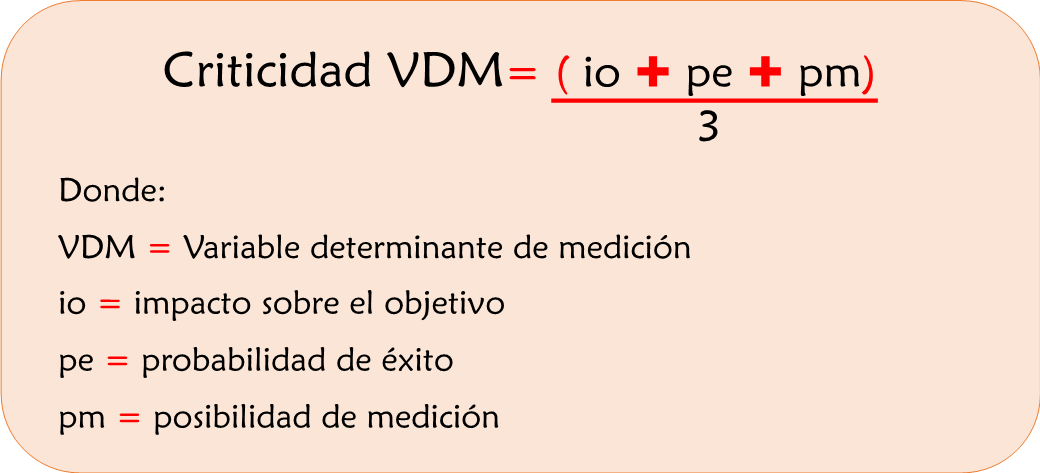
\includegraphics[width=0.6\linewidth]{Imagenes/texto_10} 

}

\caption{Ecuación para la evaluación de la criticidad de las variables determinantes de medición}\label{fig:texto10}
\end{figure}

El resultado que se obtiene de la operación anterior se ubica en una escala ordinal que va de 1 a 5, con tres rangos: \emph{``bajo''}, \emph{``medio''} y \emph{``alto''} que se describen en la \ref{tab:tablaD}. De esta manera se logra establecer el nivel de criticidad de cada variable determinante de medición.

\begin{table}

\caption{\label{tab:tablaD}*Niveles de criticidad de las variables de medición*}
\centering
\begin{tabular}[t]{l|l|l}
\hline
Valor & Nivel & Descripción\\
\hline
Entre 1 y 2,5 inclusive & Bajo & Variables que tienen menor incidencia en el cumplimiento del objetivo del proceso\\
\hline
Entre 2,5 y 3,5 inclusive & Medio & Las variables tienen una afectación intermedia en el cumplimiento del objetivo del proceso.\\
\hline
Entre 3,5 y 5 inclusive & Alto & En este rango se ubican las variables que afectan significativamente el cumplimiento del objetivo del proceso.\\
\hline
\end{tabular}
\end{table}

Una vez se tiene la evaluación de la totalidad de las variables determinantes de medición se seleccionan aquellas que obtuvieron las mayores calificaciones, en lo posible las que se encuentren en un nivel de criticidad \emph{``Alto''} para iniciar la construcción de los correspondientes indicadores de gestión.

\hypertarget{anexo-2-aplicaciuxf3n-del-modelo-de-cuantificaciuxf3n-mediciuxf3n-y-seguimiento-a-la-gestiuxf3n-de-los-procesos-a-otros-sistemas-del-siga}{%
\subsection{Anexo 2: Aplicación del modelo de cuantificación, medición y seguimiento a la gestión de los procesos a otros sistemas del siga}\label{anexo-2-aplicaciuxf3n-del-modelo-de-cuantificaciuxf3n-mediciuxf3n-y-seguimiento-a-la-gestiuxf3n-de-los-procesos-a-otros-sistemas-del-siga}}

La metodología para la cuantificación, medición y seguimiento al desempeño de los procesos que hace parte del SGC de la UNAL y que se expone en la presente guía, es replicable a los demás sistemas de gestión conforman el modelo SIGA, de igual forma el aplicativo SoftExpert permite la parametrización las particularidades de los tableros de control requeridos con el fin de sistematizar la totalidad de la información institucional en el módulo de \emph{``desempeño''}.

Para su adaptación se deberán tomar en cuenta las particularidades de cada sistema de gestión (Ambiental, Seguridad de la Información, Seguridad y Salud en el Trabajo, Gestión Documental, Laboratorios, etc.) derivadas principalmente de la normativa aplicable. A manera de ejemplo a continuación, se enuncian aspectos particulares para tener en cuenta en la medición del desempeño de algunos de los sistemas que hacen parte del modelo SIGA:

\begin{itemize}
\item
  En el caso del Sistema de Seguridad de la Información, la NTC ISO 27001:2013 \citet{ri2014tecnologia} describe en el numeral 9.1 Seguimiento, medición, análisis y evaluación, la necesidad de determinar qué se debe medir tomando en cuenta los procesos y los controles de seguridad de la información, así mismo cuáles son los métodos por usar garantizando la validez de los resultados de las mediciones del desempeño, la periodicidad y el análisis de los datos obtenidos.
\item
  Por otra parte, el Decreto 1072 de 2015 \citet{de2015decreto} señala en su Capítulo 6, Artículos 2.2.4.6.16, 2.2.4.6.17, 2.2.4.6.19, 2.2.4.6.20, 2.2.4.6.21 y 2.2.4.6.22 que se deben definir indicadores que evalúen la estructura, el proceso y los resultados del Sistema de Seguridad y Salud en el Trabajo. Así mismo establece que para la construcción de estos indicadores la entidad debe considerar aspectos como la Política de Seguridad y Salud en el Trabajo, los objetivos y metas propuestos, los planes de trabajo anuales, el plan de capacitación, el plan de atención y prevención de emergencias, el método para la identificación de peligros y evaluación y calificación de riesgos, la evaluación de las condiciones de salud de los trabajadores, el cumplimiento de normativa aplicable, entre otros.
\item
  En lo que corresponde al Sistema de Gestión Ambiental, la NTC ISO 14001:2015 \citet{cubana2004sistemas} precisa que las organizaciones deben evaluar el cumplimiento de sus requisitos legales entre otros con una frecuencia determinada e implementar acciones a partir de los resultados obtenidos.
\item
  El Modelo de Acreditación en Alta Calidad actualizado mediante el Acuerdo 02 de 2020 , establece en su artículo 20 ``\,'' Factor 4 \emph{``Mejoramiento continuo y autorregulación''} Característica 15 \emph{``Sistema interno de aseguramiento de la calidad''}, que las instituciones deben contar con indicadores de diversos tipos para hacer seguimiento a su gestión y lograr un mejoramiento continuo.
\end{itemize}

Si bien cada sistema en particular debe cumplir con ciertos requisitos para la medición de su desempeño, con el modelo de cuantificación, medición y seguimiento a la gestión desarrollado en esta guía, es posible armonizar los elementos convergentes que se mencionan en las diferentes normas, para fortalecer un sistema de indicadores institucional integrado y estructurado que se despliegue en diferentes niveles (a nivel de sistemas de gestión o a nivel de procesos).

\begin{table}

\caption{\label{tab:tablaE}*Niveles de criticidad de las variables de medición*}
\centering
\begin{tabular}[t]{l|l|l}
\hline
Valor & Nivel & Descripción\\
\hline
Entre 1 y 2,5 inclusive & Bajo & Variables que tienen menor incidencia en el cumplimiento del objetivo del proceso\\
\hline
Entre 2,5 y 3,5 inclusive & Medio & Las variables tienen una afectación intermedia en el cumplimiento del objetivo del proceso.\\
\hline
Entre 3,5 y 5 inclusive & Alto & En este rango se ubican las variables que afectan significativamente el cumplimiento del objetivo del proceso.\\
\hline
\end{tabular}
\end{table}

\begin{quote}
Elaboró: Equipo SIGA Nivel Nacional

\begin{quote}
Cargo: Analista
\end{quote}

\begin{quote}
\begin{quote}
Fecha: 28/12/2020
\end{quote}
\end{quote}

Revisó: Alberto Rodríguez Rodríguez

\begin{quote}
Cargo: Asesor DNPE
\end{quote}

Aprobó: Gloria Inés Cardona Giraldo

\begin{quote}
Cargo: Asesora VRG y Líder SIGA NN8
\end{quote}
\end{quote}

\hypertarget{referencias}{%
\chapter*{Referencias}\label{referencias}}
\addcontentsline{toc}{chapter}{Referencias}

  \bibliography{book.bib,packages.bib}

\end{document}
